\documentclass[11pt]{article}

\usepackage[utf8]{inputenc}
\usepackage{amssymb}
\usepackage{graphicx}
\usepackage{amsmath}
\usepackage{subfig}
\usepackage{hyperref}

%opening
\title{Tree Cover Variability Increases from 2005 to 2100\\ in Sub-Saharan Africa}
\author{Cody Carroll, Eric Kalosa-Kenyon, Amy Kim}

\begin{document}

\maketitle

\begin{abstract}
This report fufills the requirements for the final project in Time Series
    Analysis (STA237A). The authors report on the behavior of simulated tree
    cover between the years of 2005 and 2100. The preliminary analysis using
    common time series methods is followed by changepoint and spacio-temporal
    analyses.

    All authors contributed equally to this work.
\end{abstract}

\section{Introduction}
Climate change is driven by anthropogenic carbon forcing. Predicated on this
inconvenient reality, the Intergovernmental Pannel on Climate Change has
developed representative carbon forcing pathways (RCPs) to coordinate
climate research. Ensembles of computer simulations are run using pre-selected
RCPs and calibrated using historical observations. These simulations are
realizations of gridded meteorological PDEs in the Community Climate Model
System (CCMS). The CCMS has 5 components and a coupler: atmosphere, sea, land,
sea ice, and land ice. These modules each influence the global climate and each
module generates output for subsequent analysis.

In this report, we interrogate the output of the land module both globally and
over a single location in Sub-Saharan Africa. The ensemble used to generate this
data follows the RCP4.5 carbon pathway. Roughly, this pathway captures the
atmospheric carbon concentration induced by peak carbon emissions around 2035
with a decrease thereafter. We are interested to understand how a highly
productive region's tree cover responds to this RCP. The location in question is 

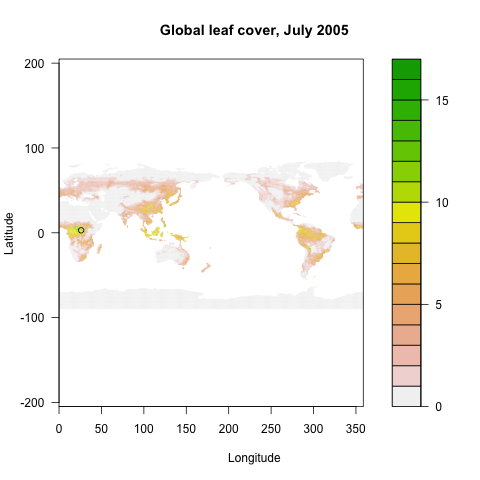
\includegraphics{../img/LAI_global_t0.png}

LAI is unitless quantity (leaf area ($m^2$))/(ground area ($m^2$))
"Comparative Physiological Studies on the Growth of Field Crops" Watson 1947 Annals of Botany
Bounded below by 0, above by physiological limits

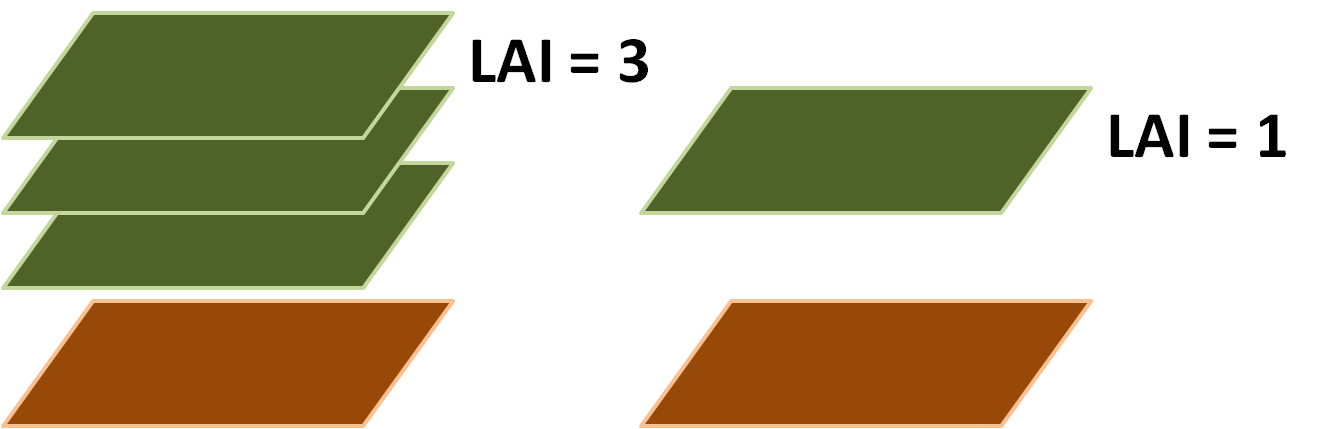
\includegraphics{../img/lai.png}\\
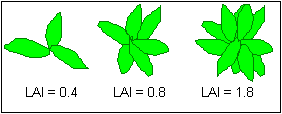
\includegraphics{../img/lai2.png}

The raw data at a single location is presented in the figure below:
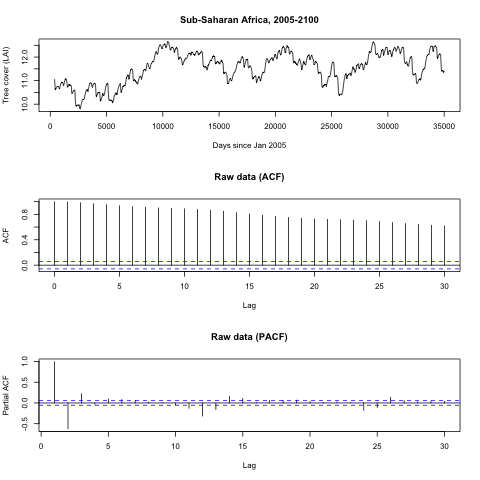
\includegraphics{../img/pacf_acf_raw.png}

The detrended data at a single location is presented in the figure below:
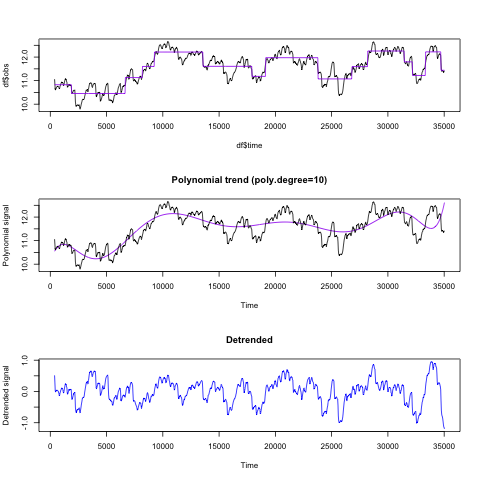
\includegraphics{../img/detrended_acf_pacf.png}

The variance-standardized data at a single location is presented in the figure
below:
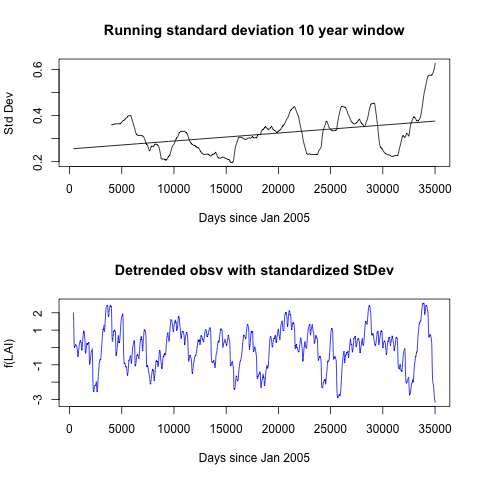
\includegraphics{../img/standatdized_var_LAI.png}

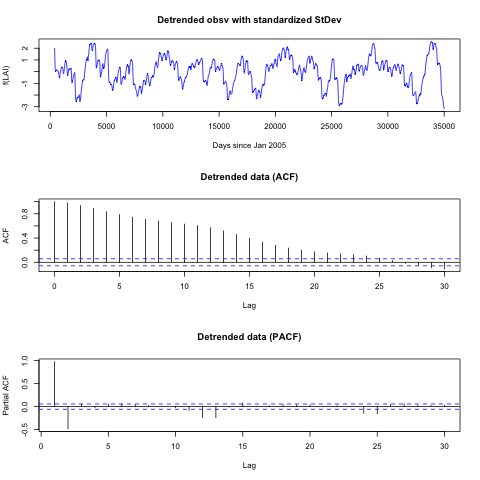
\includegraphics{../img/detrended_stdzd_acf_pacf.png}

The differenced data at a single location is presented in the figure below:
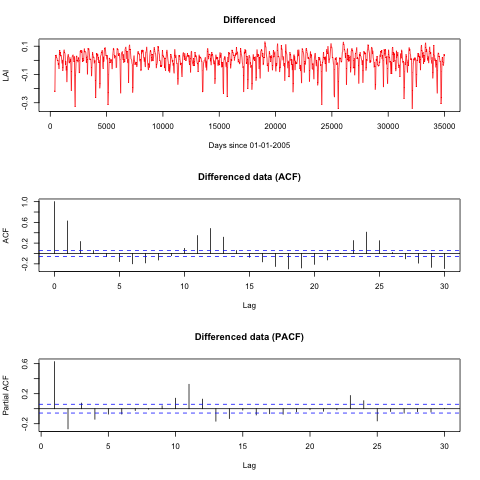
\includegraphics{../img/differenced_acf_pacf.png}

The deseasoned data at a single location is presented in the figure below:
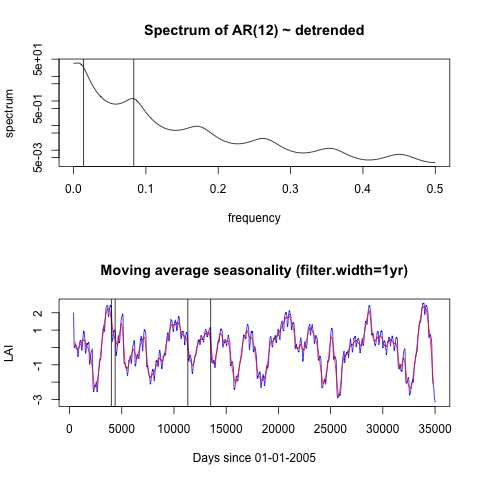
\includegraphics{../img/deseasonalization_spectrum.png}
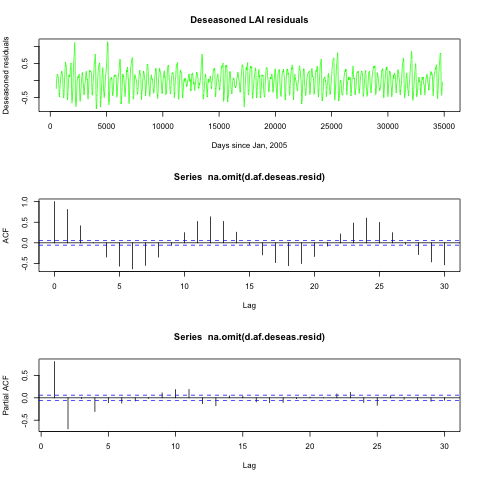
\includegraphics{../img/deseasonalization_resid.png}
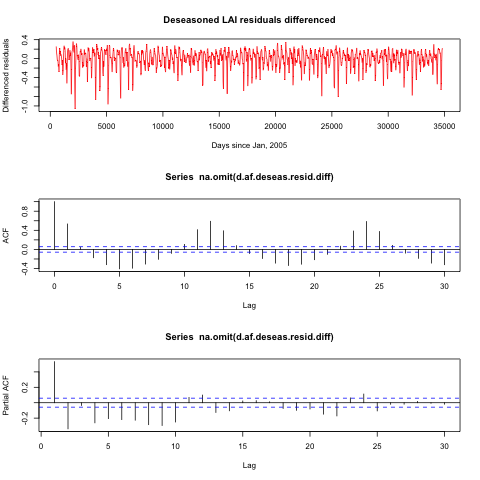
\includegraphics{../img/deseasonalization_resid_difference.png}
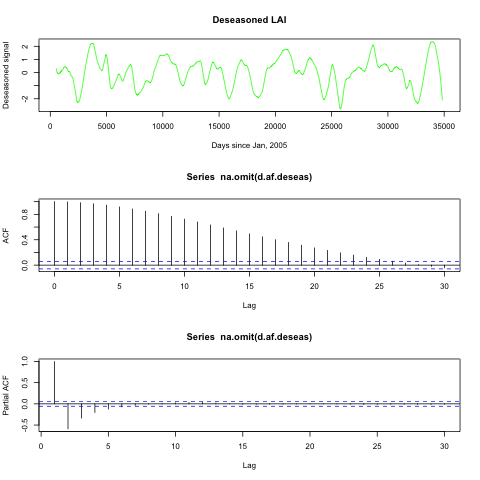
\includegraphics{../img/deseasonalization.png}

The fit of and simulation from an AR(4) to the deseasoned data is presented
below:
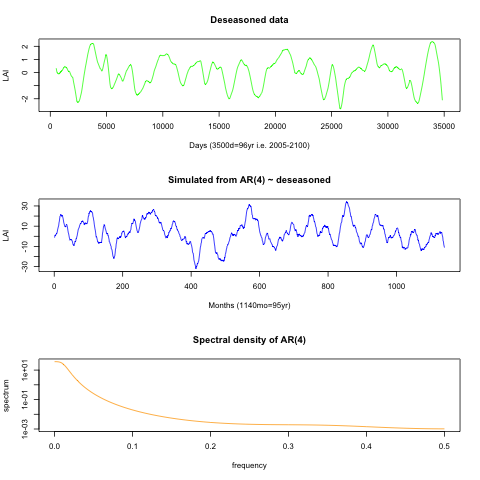
\includegraphics{../img/ar_sim.png}


\section{Changepoint}

Instead of dealing with the non-stationarity of our series by differencing and using the ARIMA framework, another approach is to notice that there are specific points in time where the time series changes behavior in one fell swoop. An example of this is around the year 2025, where the series jumps up to a mean level of around 11.75 and stays there. Figure 1 illustrates this "jump" with a red dashed line.
\begin{figure}[h]
	\centering
	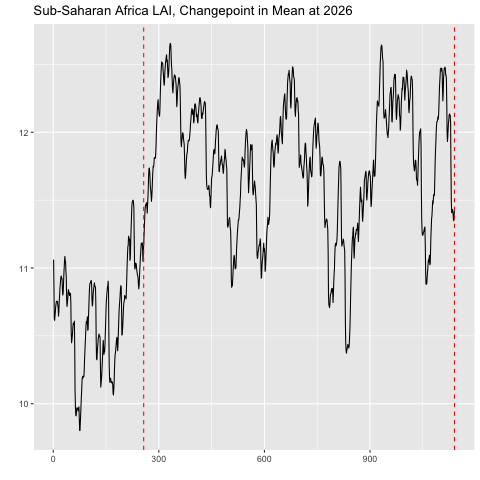
\includegraphics[width=5in, height=4.5in]{../img/changepoint_LAI.png}
	\caption{LAI TS}
\end{figure}

This point in time is called a changepoint. We give a short introduction on changepoint detection methods.\clearpage
\noindent { \sf 1.1. \quad Changepoint Detection} Conceptually, for data $Z_1,...,Z_n$, a changepoint $\tau$ is a point in time, such that $Z_1,...,Z_\tau$ differ from  $Z_\tau+1,...,Z_n$. For the sake of illustration, we take a simple example. Assume the parametric form
\begin{equation*}
	Z_t|\theta_t\sim N(\theta_t,1) \tag*{where $\theta_t=1 ~\text{if}~ t\leq\tau$ and $\theta_t=0 ~\text{if}~ t>\tau$}.
\end{equation*} An example of such a process is depicted in Figure 2.
\begin{figure}[h]
	\centering
	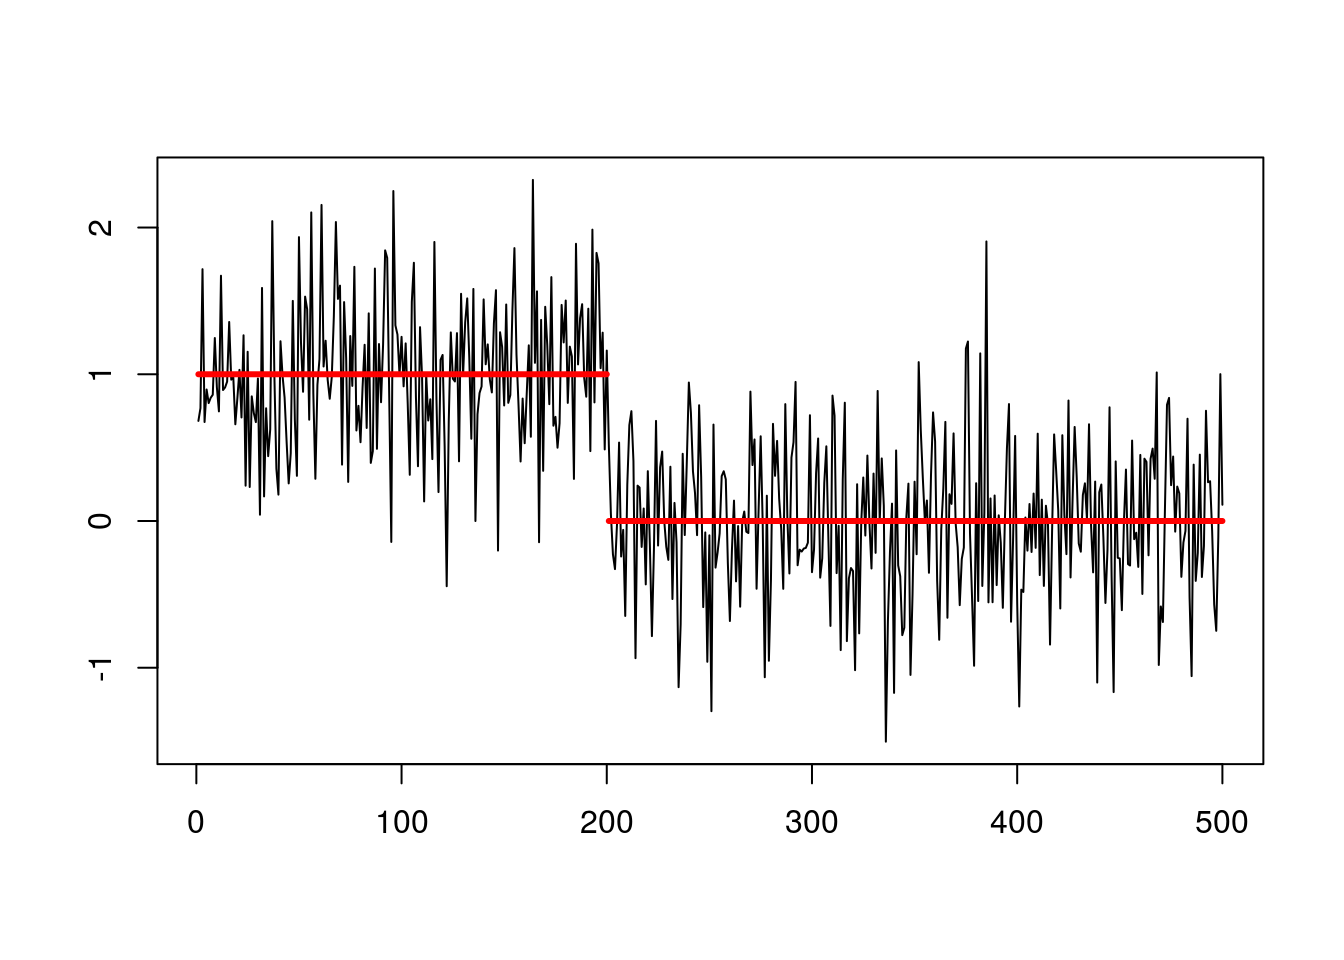
\includegraphics[width=0.75\linewidth]{../img/changepointex.png}
	\caption{Example of a Changepoint}
\end{figure}

It's intuitively clear from the picture that the change occurs at $\tau=200$, but how do we detect where a changepoint occurs, mathematically? One approach is to use a Likelihood Ratio Test. We state the hypotheses as: 
\begin{equation*}
	H_0:\theta_t=\theta~ \forall~ t \quad\text{vs.} \quad H_1:\theta_t=\theta_1,~t\leq\tau;~ \theta_t=\theta_2,~t>\tau 
\end{equation*}
To construct the likelihood ratio statistic, we need to maximize the likelihood under the null and alternative.  We let $p(\cdot)$ be the probability density function associated with the distribution of the data and $\hat{\theta}$ is the maximum likelihood estimate of the parameters. Under $H_0$, the maximum log-likelihood is $\log p(y_{1:n}|\hat{\theta})$.
Under $H_1$ with a changepoint $\tau$, the maximum log-likelihood is $ML(\tau) = \log p(y_{1:\tau}|\hat{\theta}_1) +  \log p(y_{\tau+1:n}|\hat{\theta}_2)$. Therefore the likelihood ratio statistic is:
\begin{equation*}
	\Lambda(\tau)=\dfrac{\max_\tau ML(\tau)}{\log p(y_{1:n}|\hat{\theta})}
\end{equation*}
A more commonly used version of this statistic is the log-LR statistic:
\begin{equation*}
2\log\Lambda(\tau)=2\left[\max_\tau ML(\tau)-\log p(y_{1:n}|\hat{\theta})\right]\
\end{equation*}
We compare this statistic with a cut-off value, $\lambda$. If $LR>\lambda$, then we reject $H_0$ and estimate the changepoint as 
\begin{equation*}
\hat{\tau}=\arg\max_\tau LR(\tau)
\end{equation*}
There are many different ways to select $\lambda$. Selecting an optimal value of $\lambda$ remains an open research topic in changepoint analysis. We use the package 'changepoint' to investigate if our LAI time series has a changepoint, using a specific $\lambda$ value that takes into consideration the inherent correlation between observations of a time series.
\begin{figure}
	\centering
	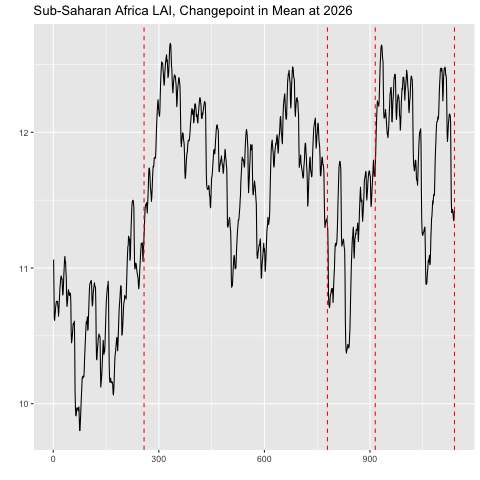
\includegraphics[width=0.55\linewidth]{../img/multi_changepoint_LAI.png}
	\caption{LAI TS}
\end{figure}
We find an estimated changepoint of $\hat{\tau}= 237$ months after Jan. 2005, i.e. 2026 is when LAI experiences a changepoint in mean. Looking at the series after 2026 though, we suspect there may be more time points. So we segment the series and iterate the changepoint estimation. We need to consider multiple testing since we are doing several tests now..



\section{Principal Component Analysis}
\paragraph{} 
We have done the time series analysis for the one location, and we can expand our analysis into global scale. This becomes the analysis of space-time with a large dataset (12818 locations and 1140 time points). In order to extract the underlying trends, we can consider Principal Component Analysis for examining both the spatial and temporal variation here. 

Principal component: Temporal pattern (true values x loadings) vs. loadings of each principal components: Spatial Pattern - eigenvectors
\paragraph{Principal Component Analysis}
\begin{equation}
\mathbf{Z}(s,t) = \mathbf{U}\mathbf{\Lambda}\mathbf{V}^T
\end{equation}
where $\mathbf{U}$ is a $T \times k$ orthogonal matrix with columns $\mathbf{u}_j, \mathbf{V}$ is a $S \times k$ orthogonal matrix with columns $\mathbf{v}_j$ and $\mathbf{\Lambda}$ is a $k \times k$ diagonal matrix with diagonal entries $\lambda_j$. This $\mathbf{Z}$: 
\begin{equation}
\mathbf{Z}(s,t)  = \begin{pmatrix}
z(s_1, t_1) & z(s_2, t_1) & z(s_3, t_1) & \dots & z(s_{12818}, t_1) \\
z(s_1, t_2) & z(s_2, t_2) & z(s_3, t_2) & \dots & z(s_{12818}, t_2) \\
\vdots & \vdots & \vdots & \ddots & \vdots\\
z(s_1, t_{1140}) & z(s_2, t_{1140}) & z(s_3, t_{1140}) & \dots & z(s_{12818}, t_{1140})\\ 
\end{pmatrix}
\end{equation}

We decide to report PCA on a detrend dataset~\footnote{We used cubic splines for each time series to extract variations} since its first few Principal Components(PCs) have more cumulative explained variances. We mainly examine the first Principal Component(PC) since it explains 43\% of variances and others do less then 10\% (Table~\ref{table:detrendprop})~\footnote{419 PCs achieve to explain 90\% of variations.}.

%rotation	
%the matrix of variable loadings (i.e., a matrix whose columns contain the eigenvectors). The function princomp returns this in the element loadings.
%x	
%if retx is true the value of the rotated data (the centred (and scaled if requested) data multiplied by the rotation matrix) is returned. Hence, cov(x) is the diagonal matrix diag(sdev^2). For the formula method, napredict() is applied to handle the treatment of values omitted by the na.action.
\subsection{Spatial Pattern}
Spatial pattern explains how strong the PCs depend on some locations, and it is represented by the loadings of each principal components. The mean spatial structure, Figure~\ref{fig:scalepcade}, indicates locations known forest area higher mean values(red) and desert areas have lower values (blue).  We can interpret PC1 implies main variance across the all locations and over the 95 years, Figure~\ref{fig:pc1}. It shows forest areas have negative effects(blue) and infertile lands have positive effects(red) which contracts to mean structure. 
\begin{figure}
	\centering
	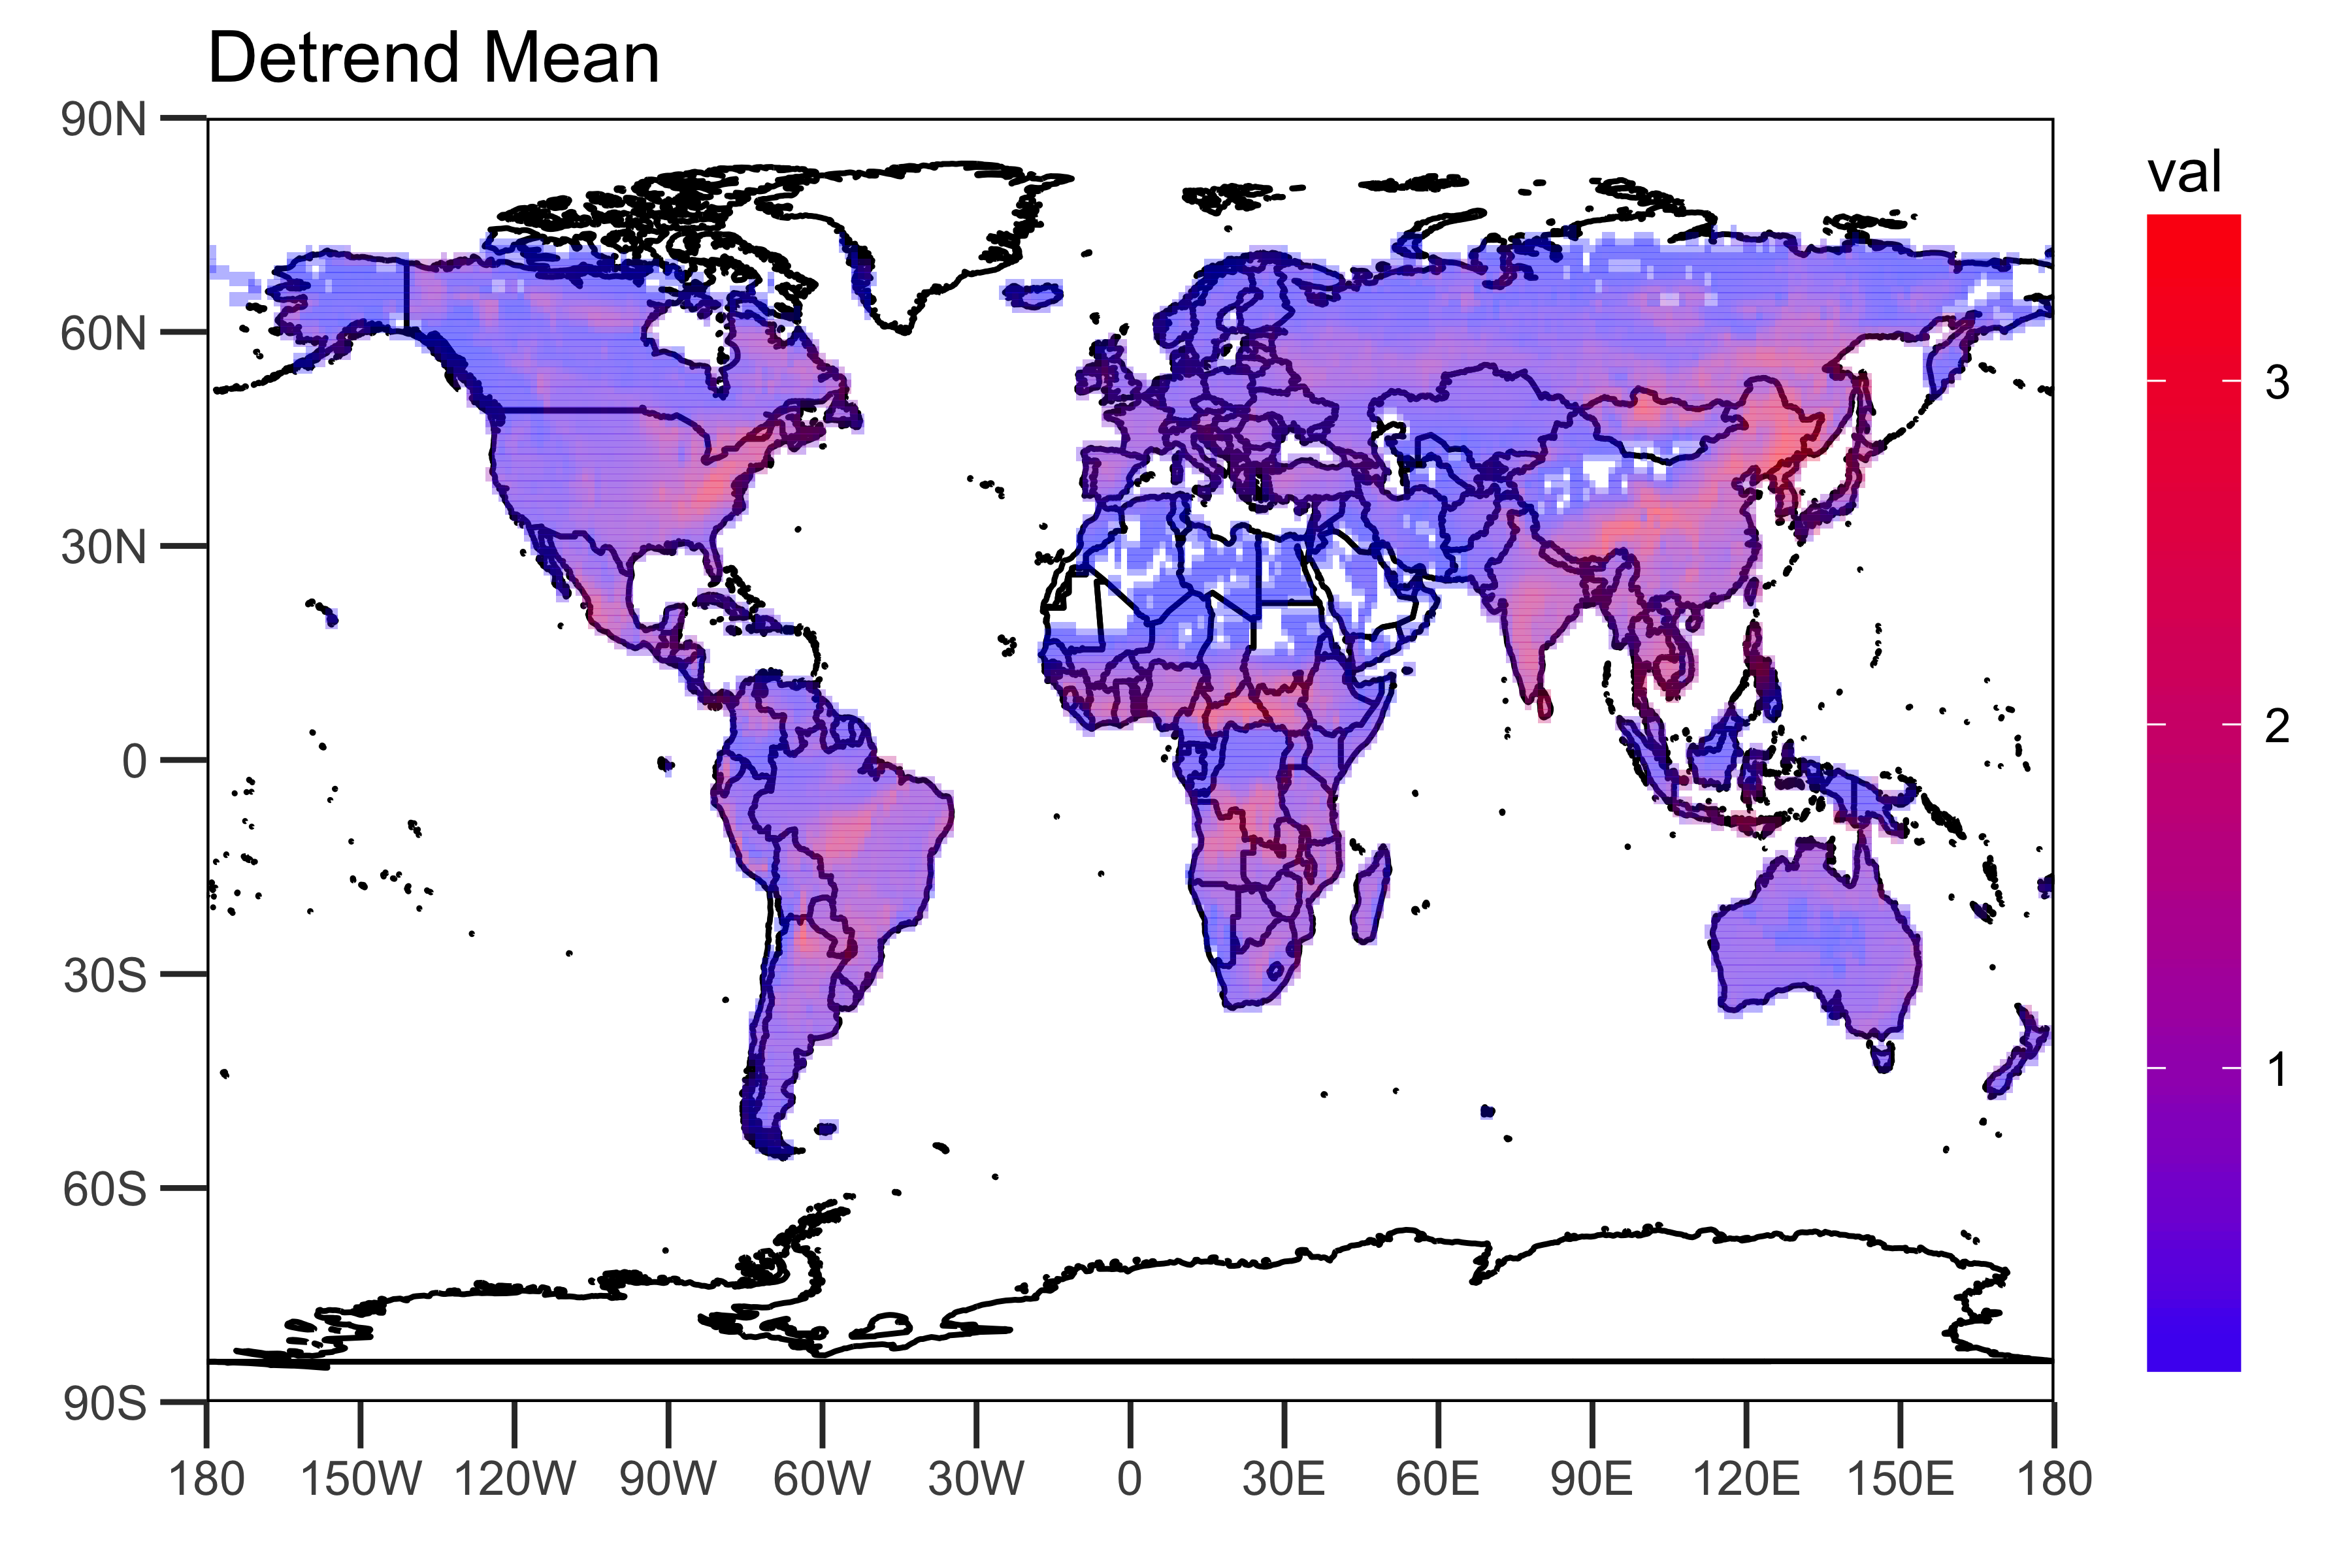
\includegraphics[width=0.7\linewidth]{../img/Scale_PCA_de}
	\caption{Overall Spatial Mean}
	\label{fig:scalepcade}
\end{figure}

\begin{figure}
	\centering
	{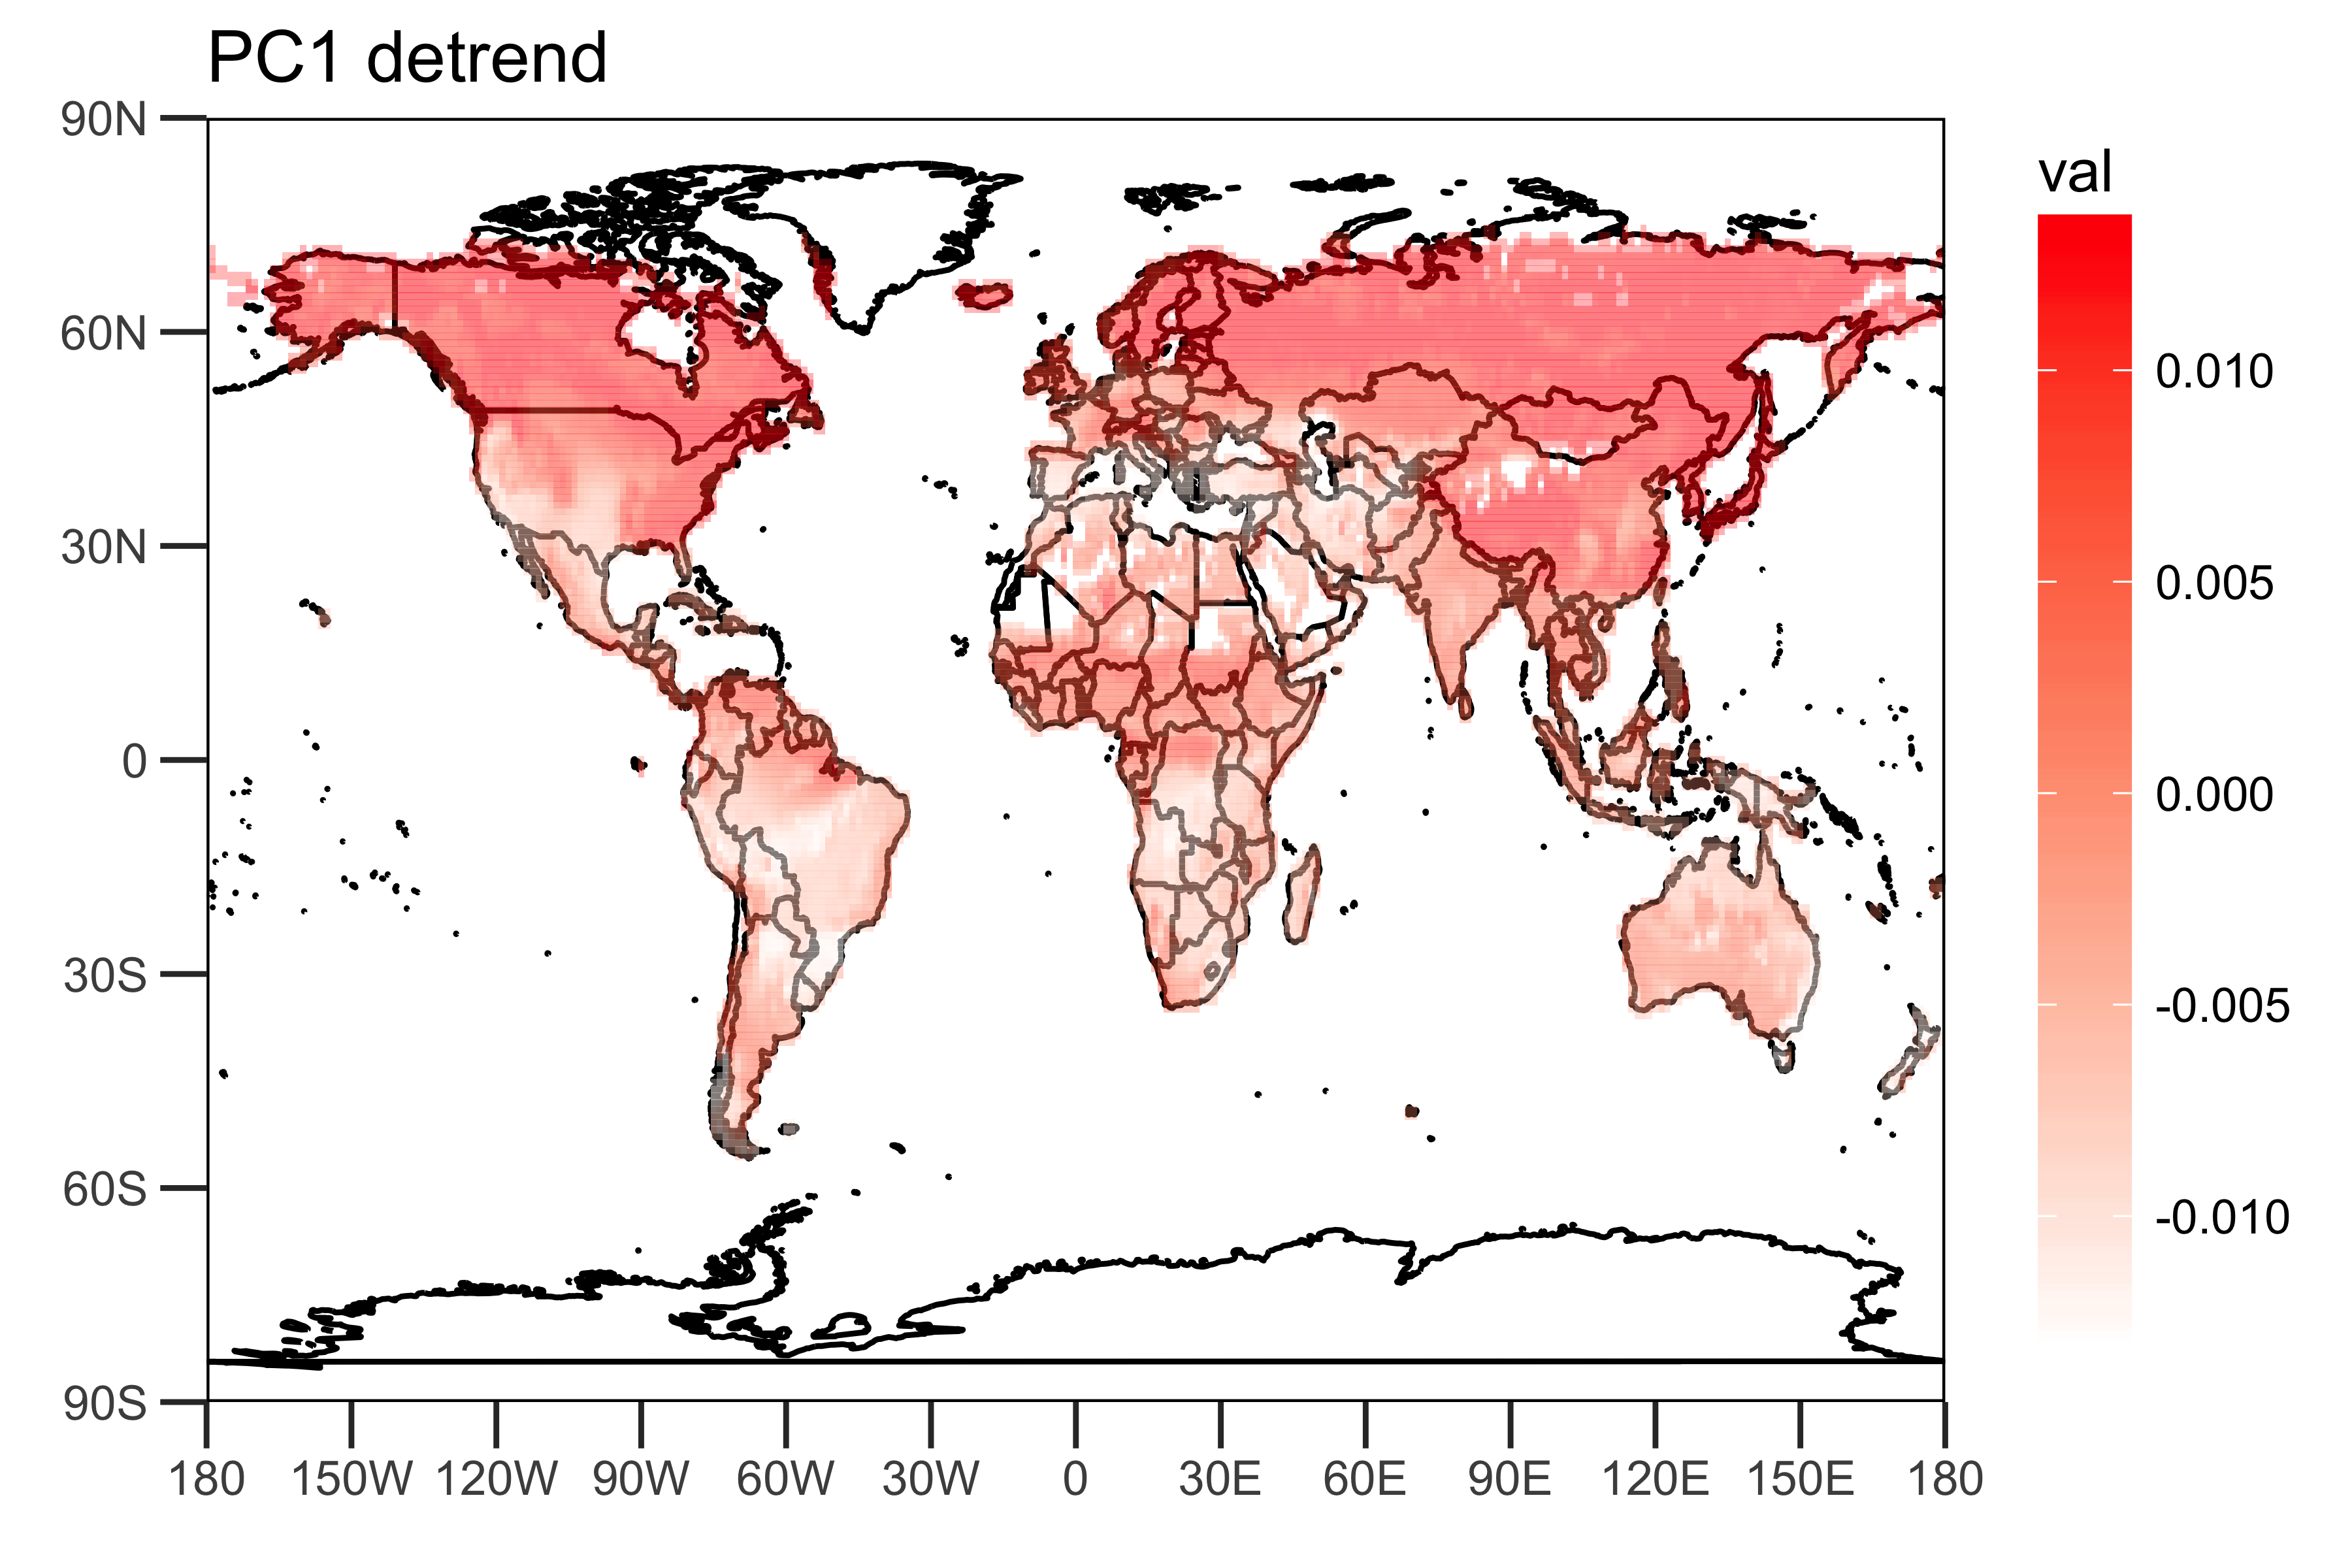
\includegraphics[width=0.7\linewidth]{../img/loading_PC1_de}}\label{fig:pc1-spatial}
%	\subfloat[PC 1]{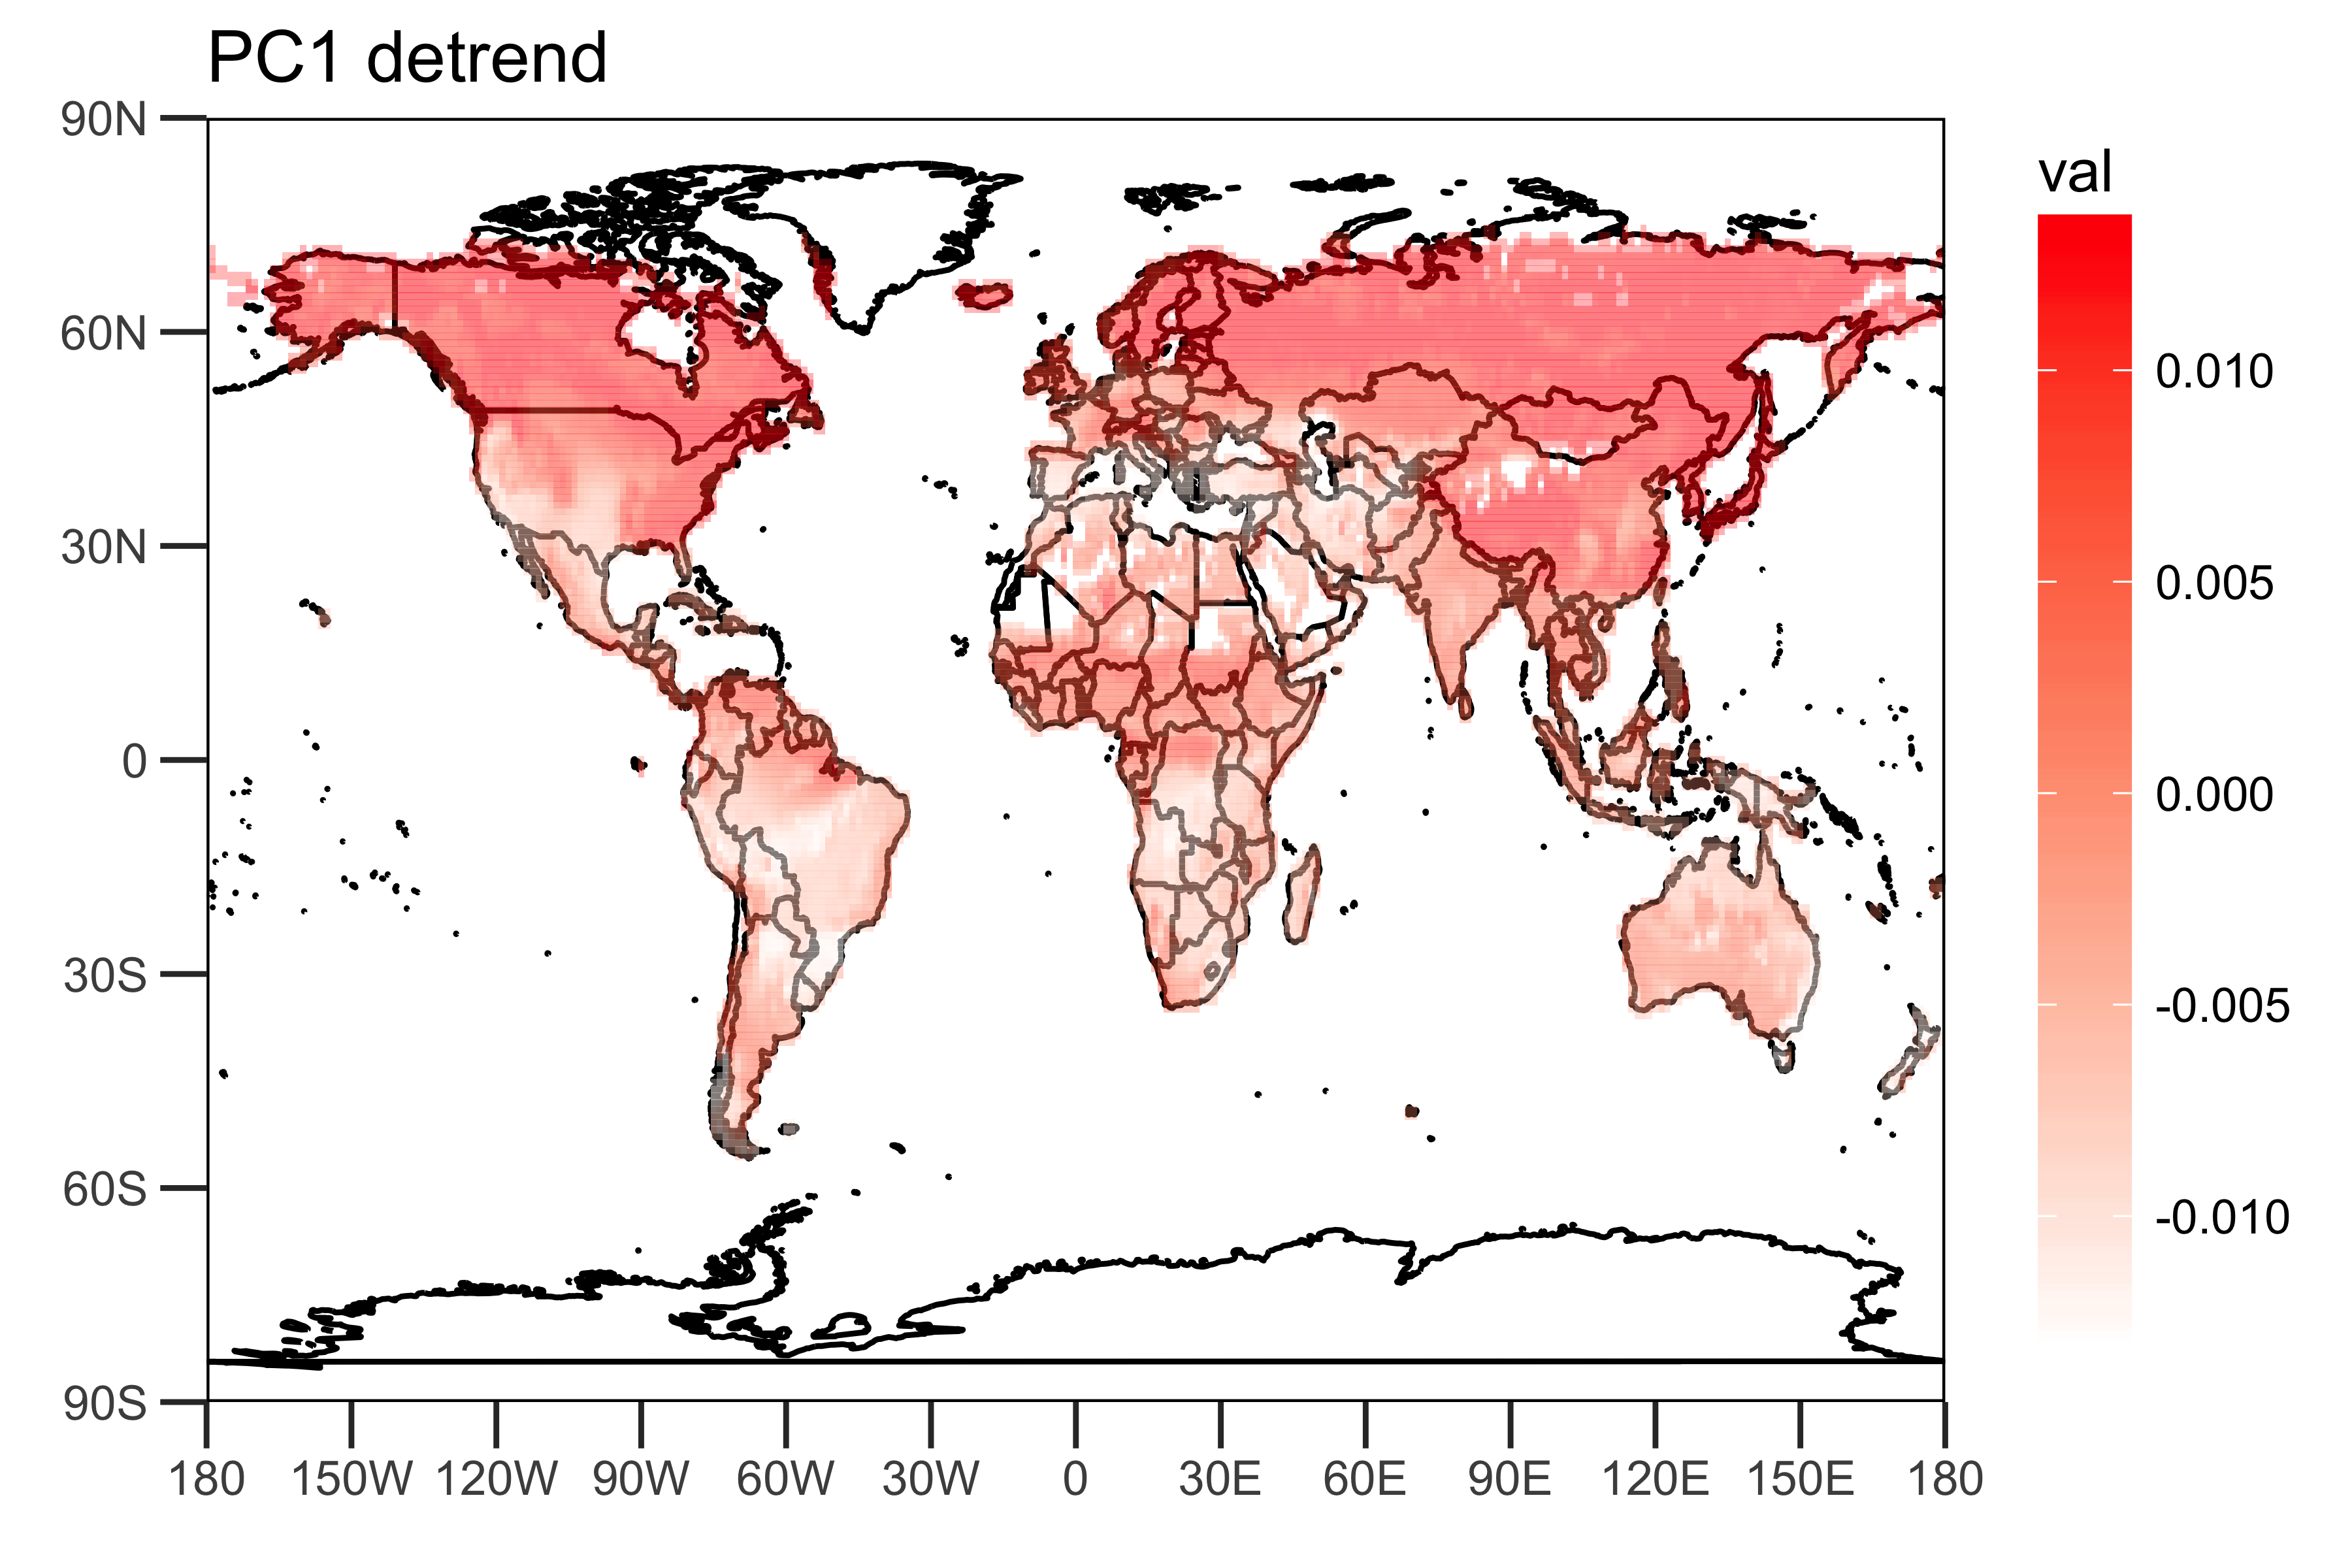
\includegraphics[width=0.45\linewidth]{../img/loading_PC1_de}}\label{fig:pc1}
%	\hfill
%	\subfloat[PC 2]{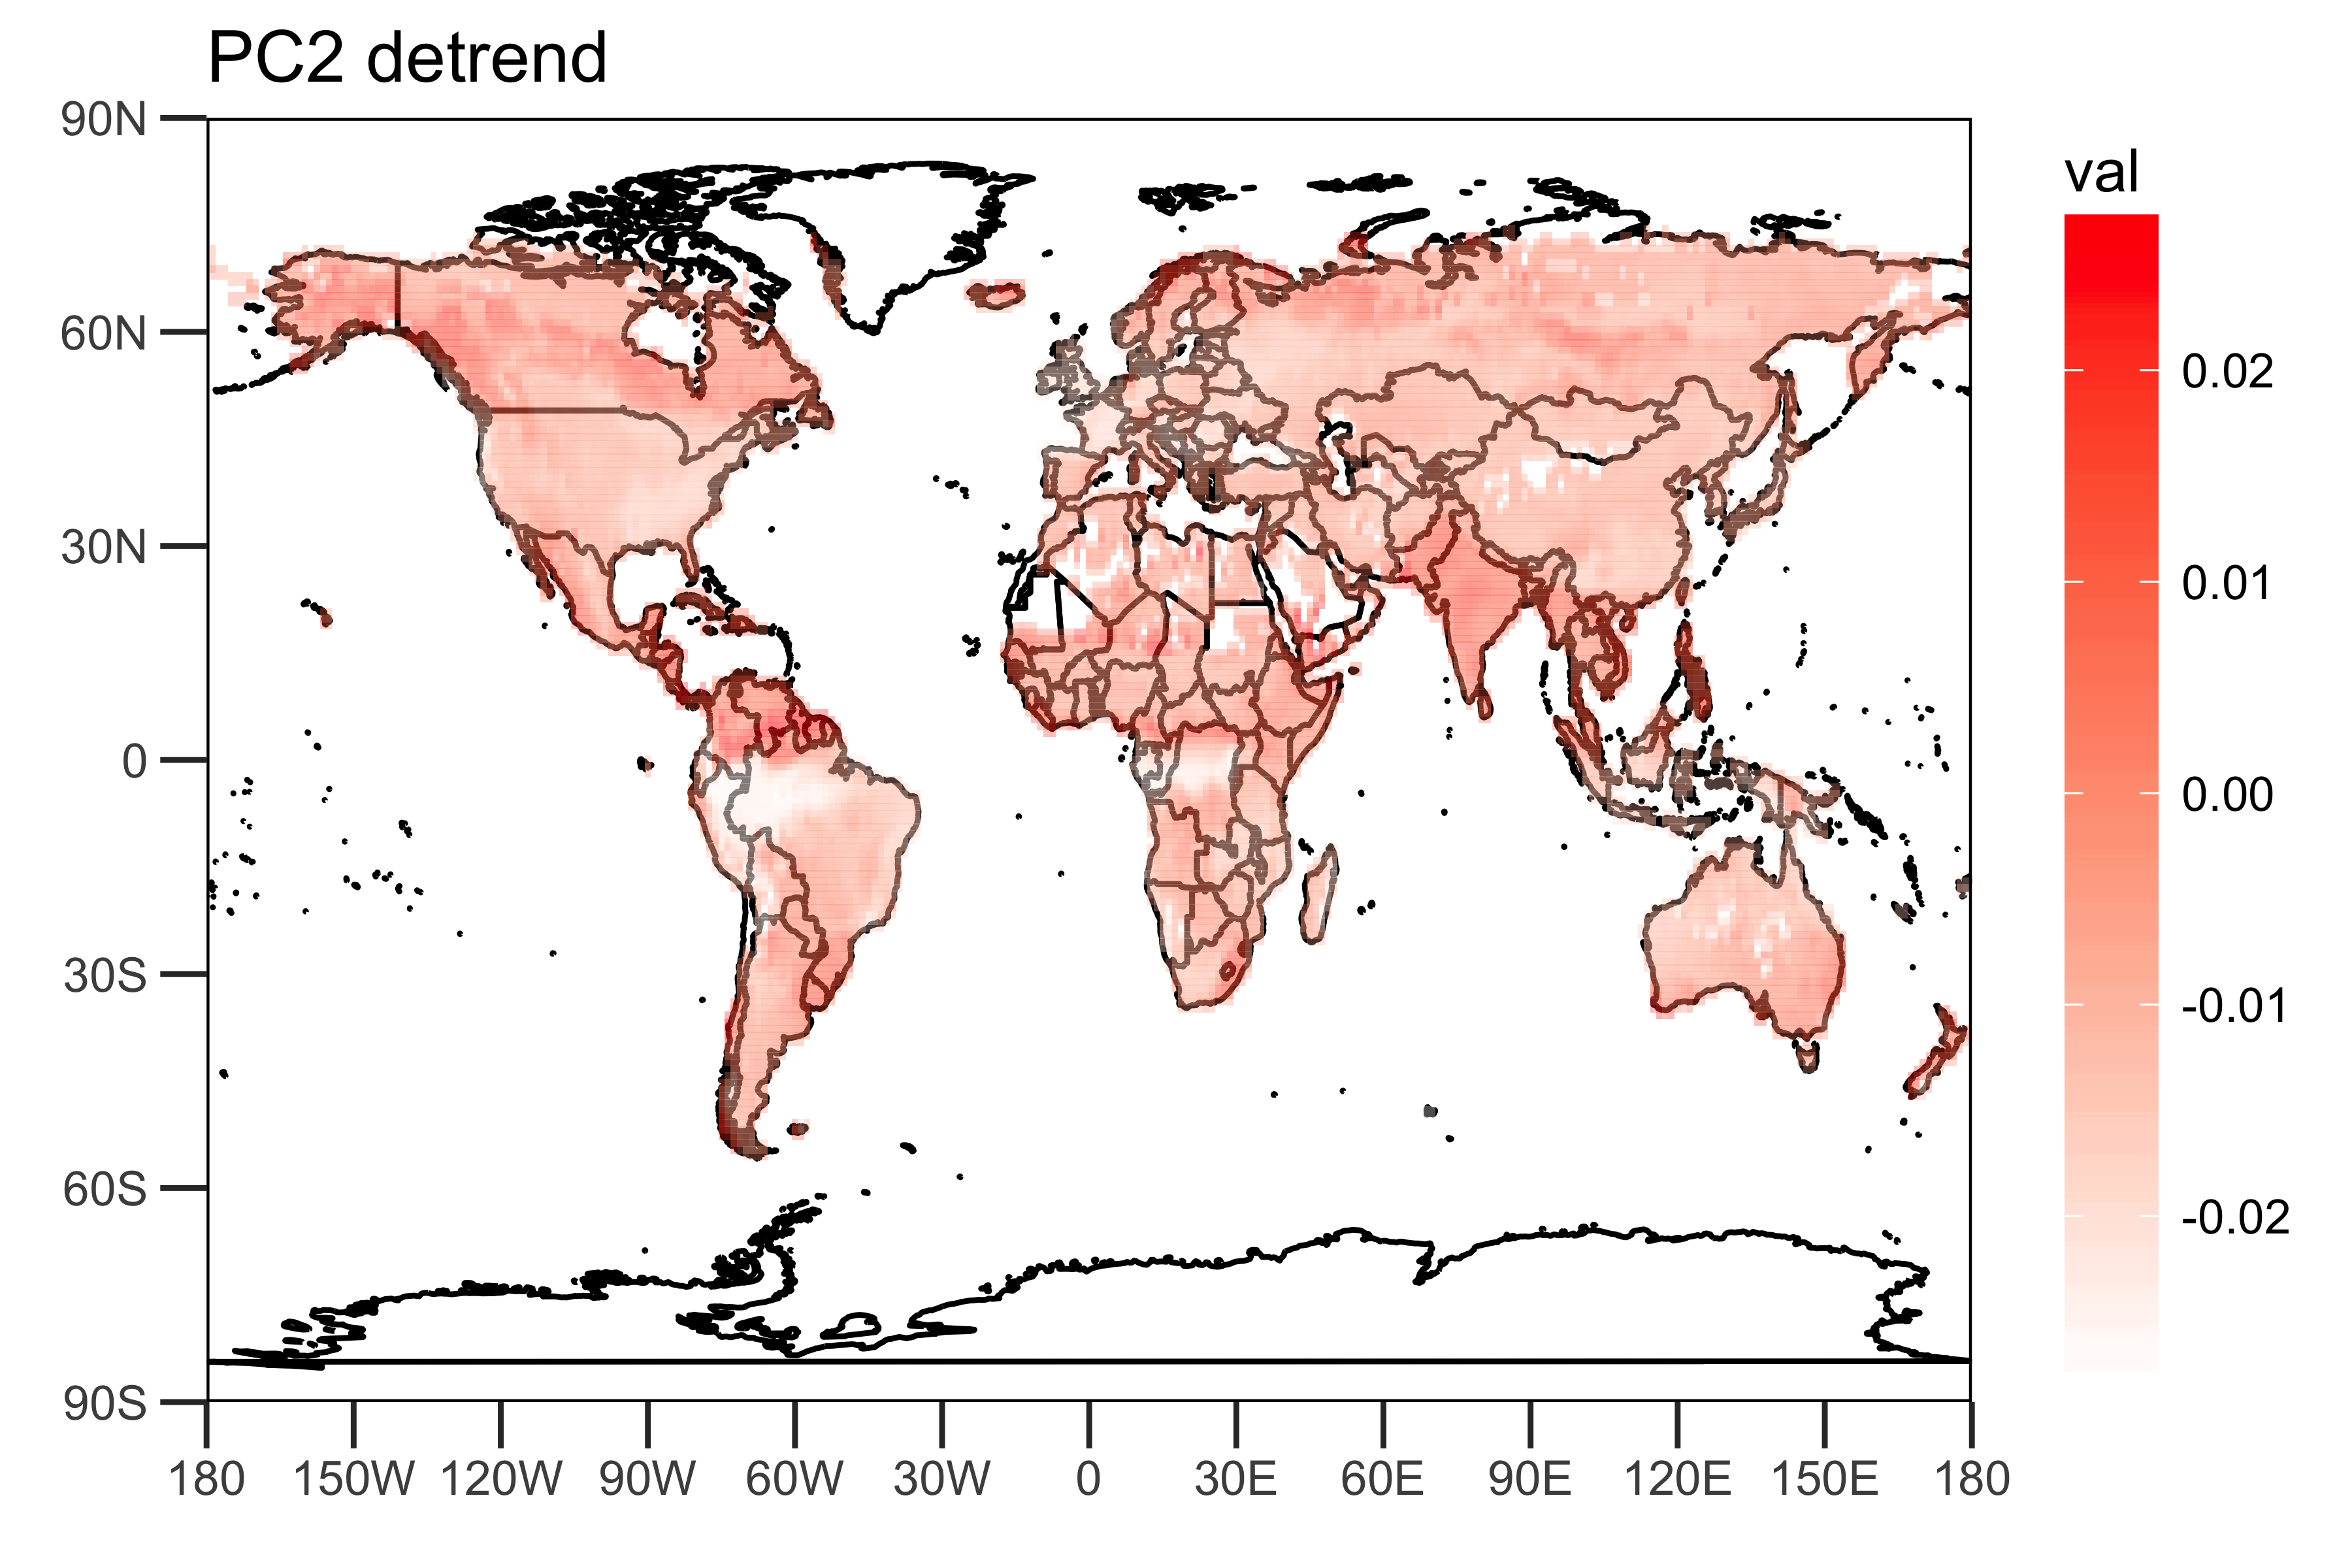
\includegraphics[width=0.45\linewidth]{../img/loading_PC2_de}}\label{fig:pc2}
%	\subfloat[PC 3]{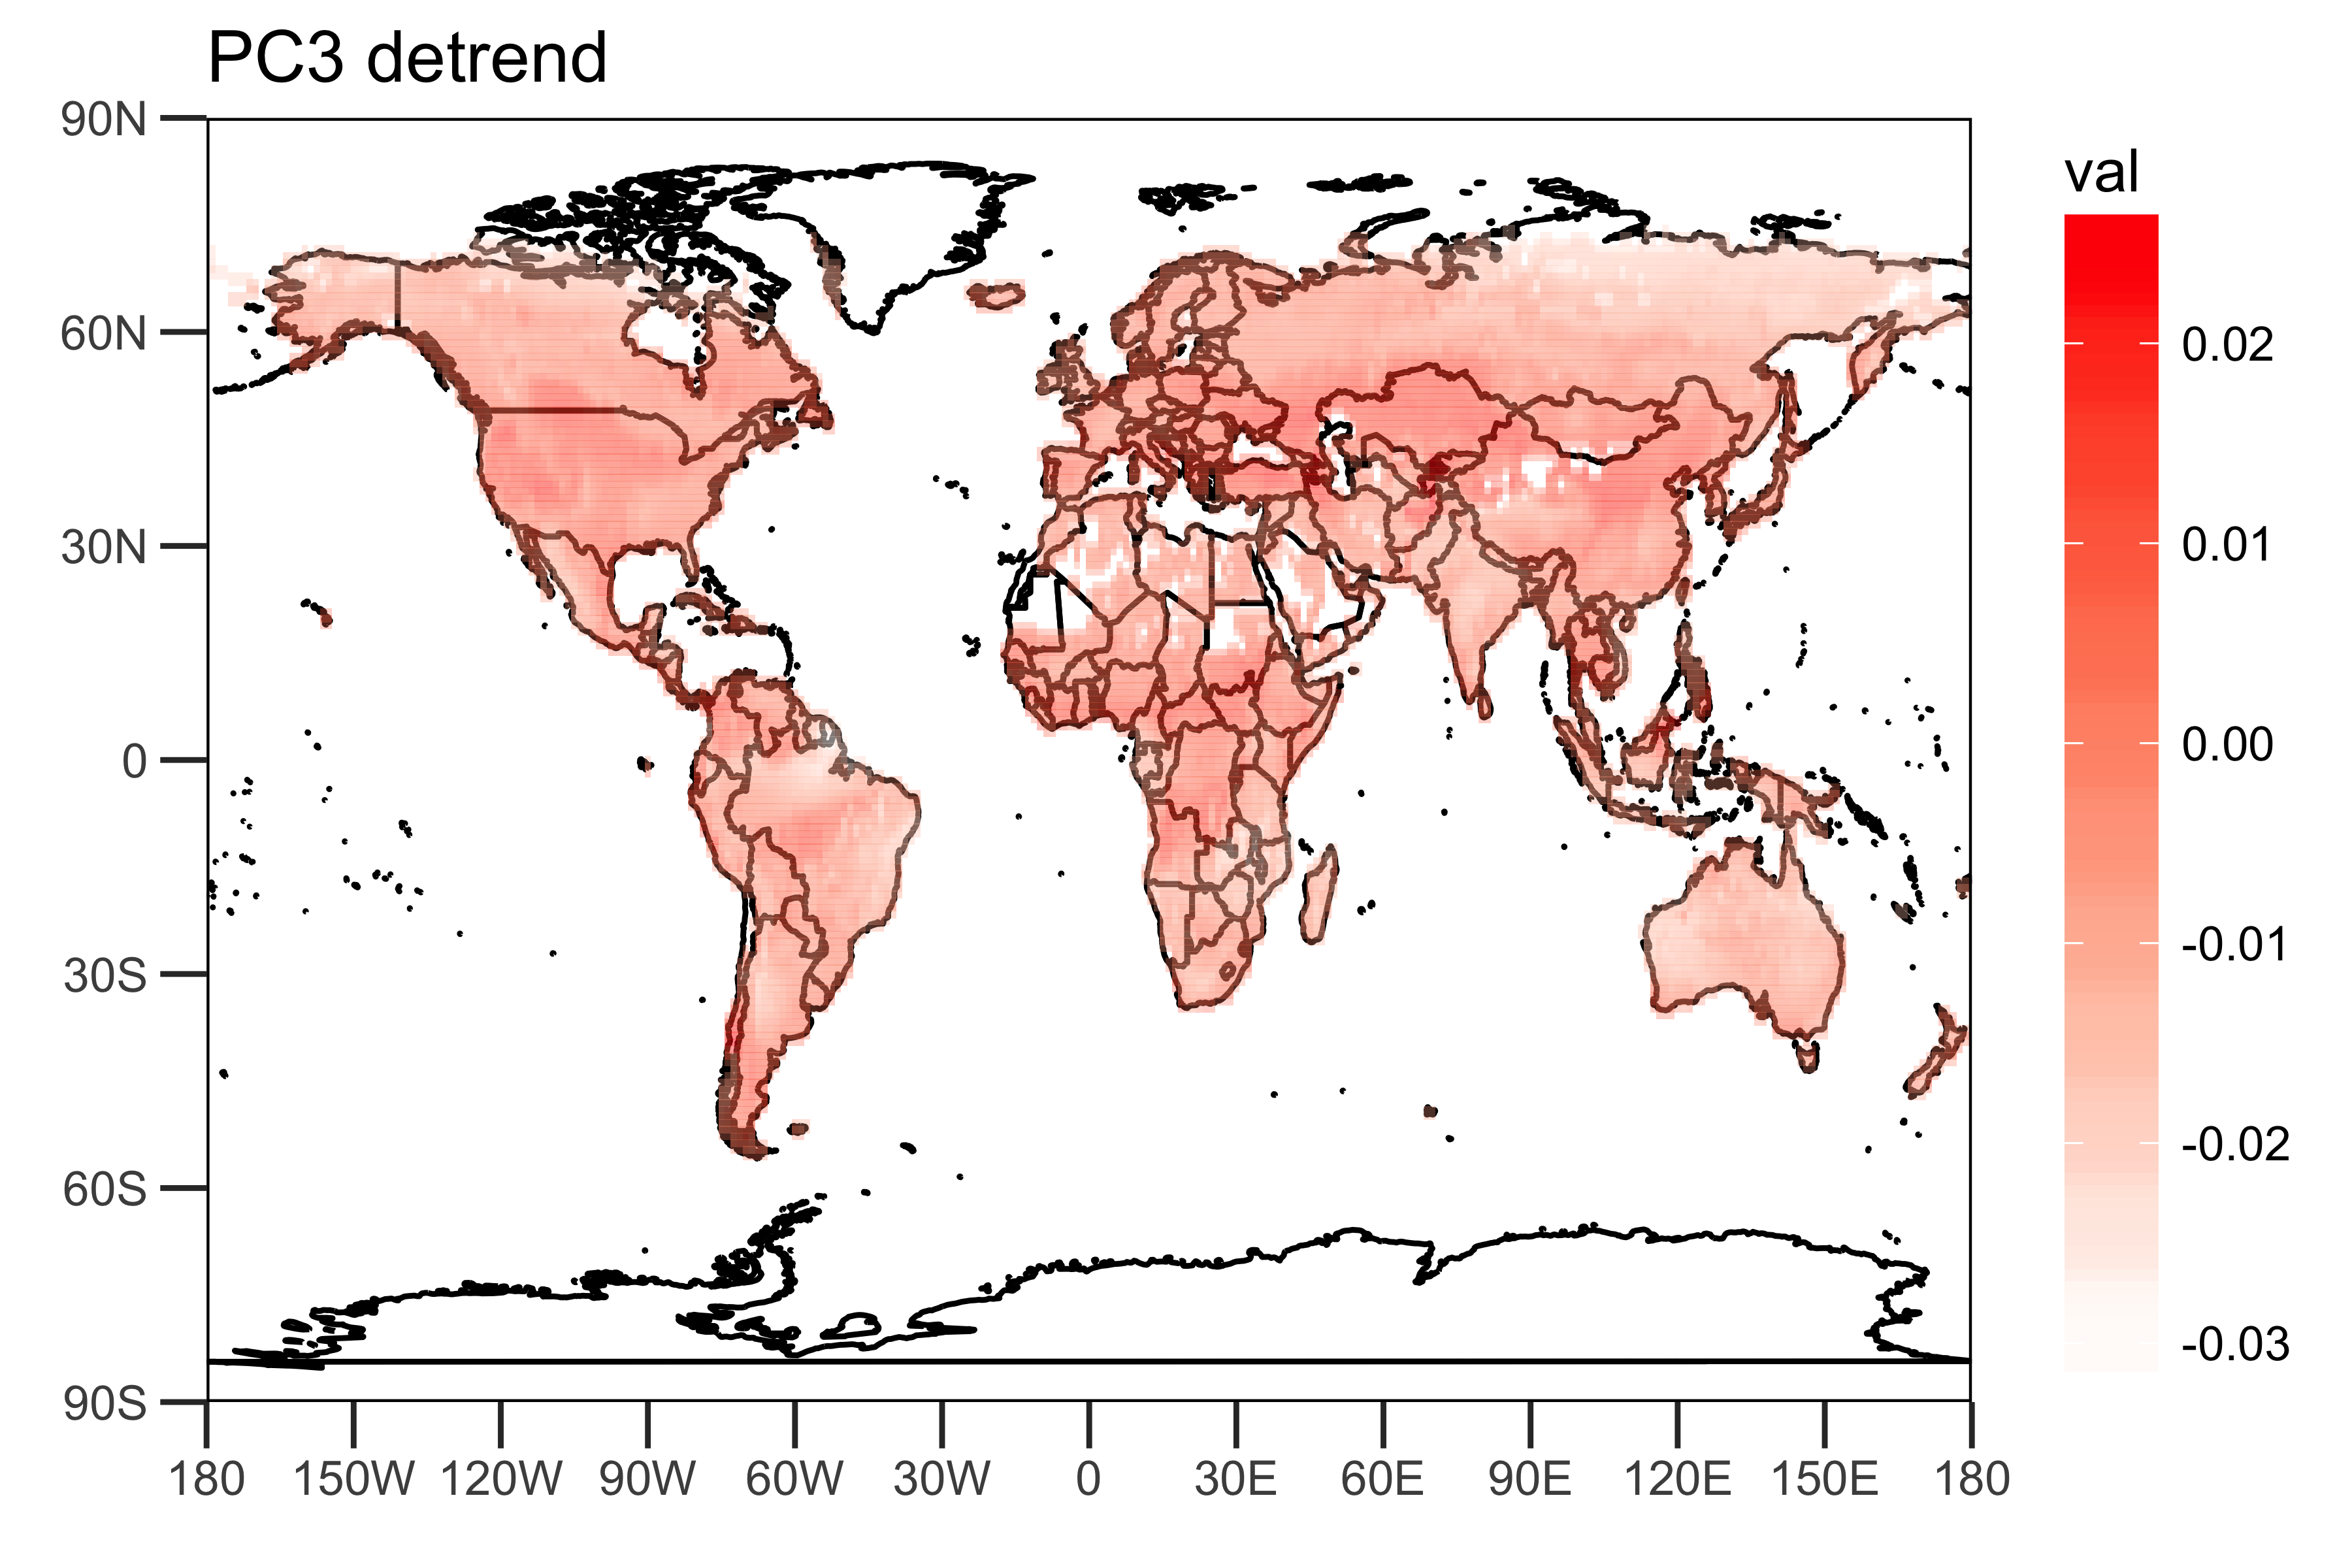
\includegraphics[width=0.45\linewidth]{../img/loading_PC3_de}}\label{fig:pc3}
%	\hfill
%	\subfloat[PC 4]{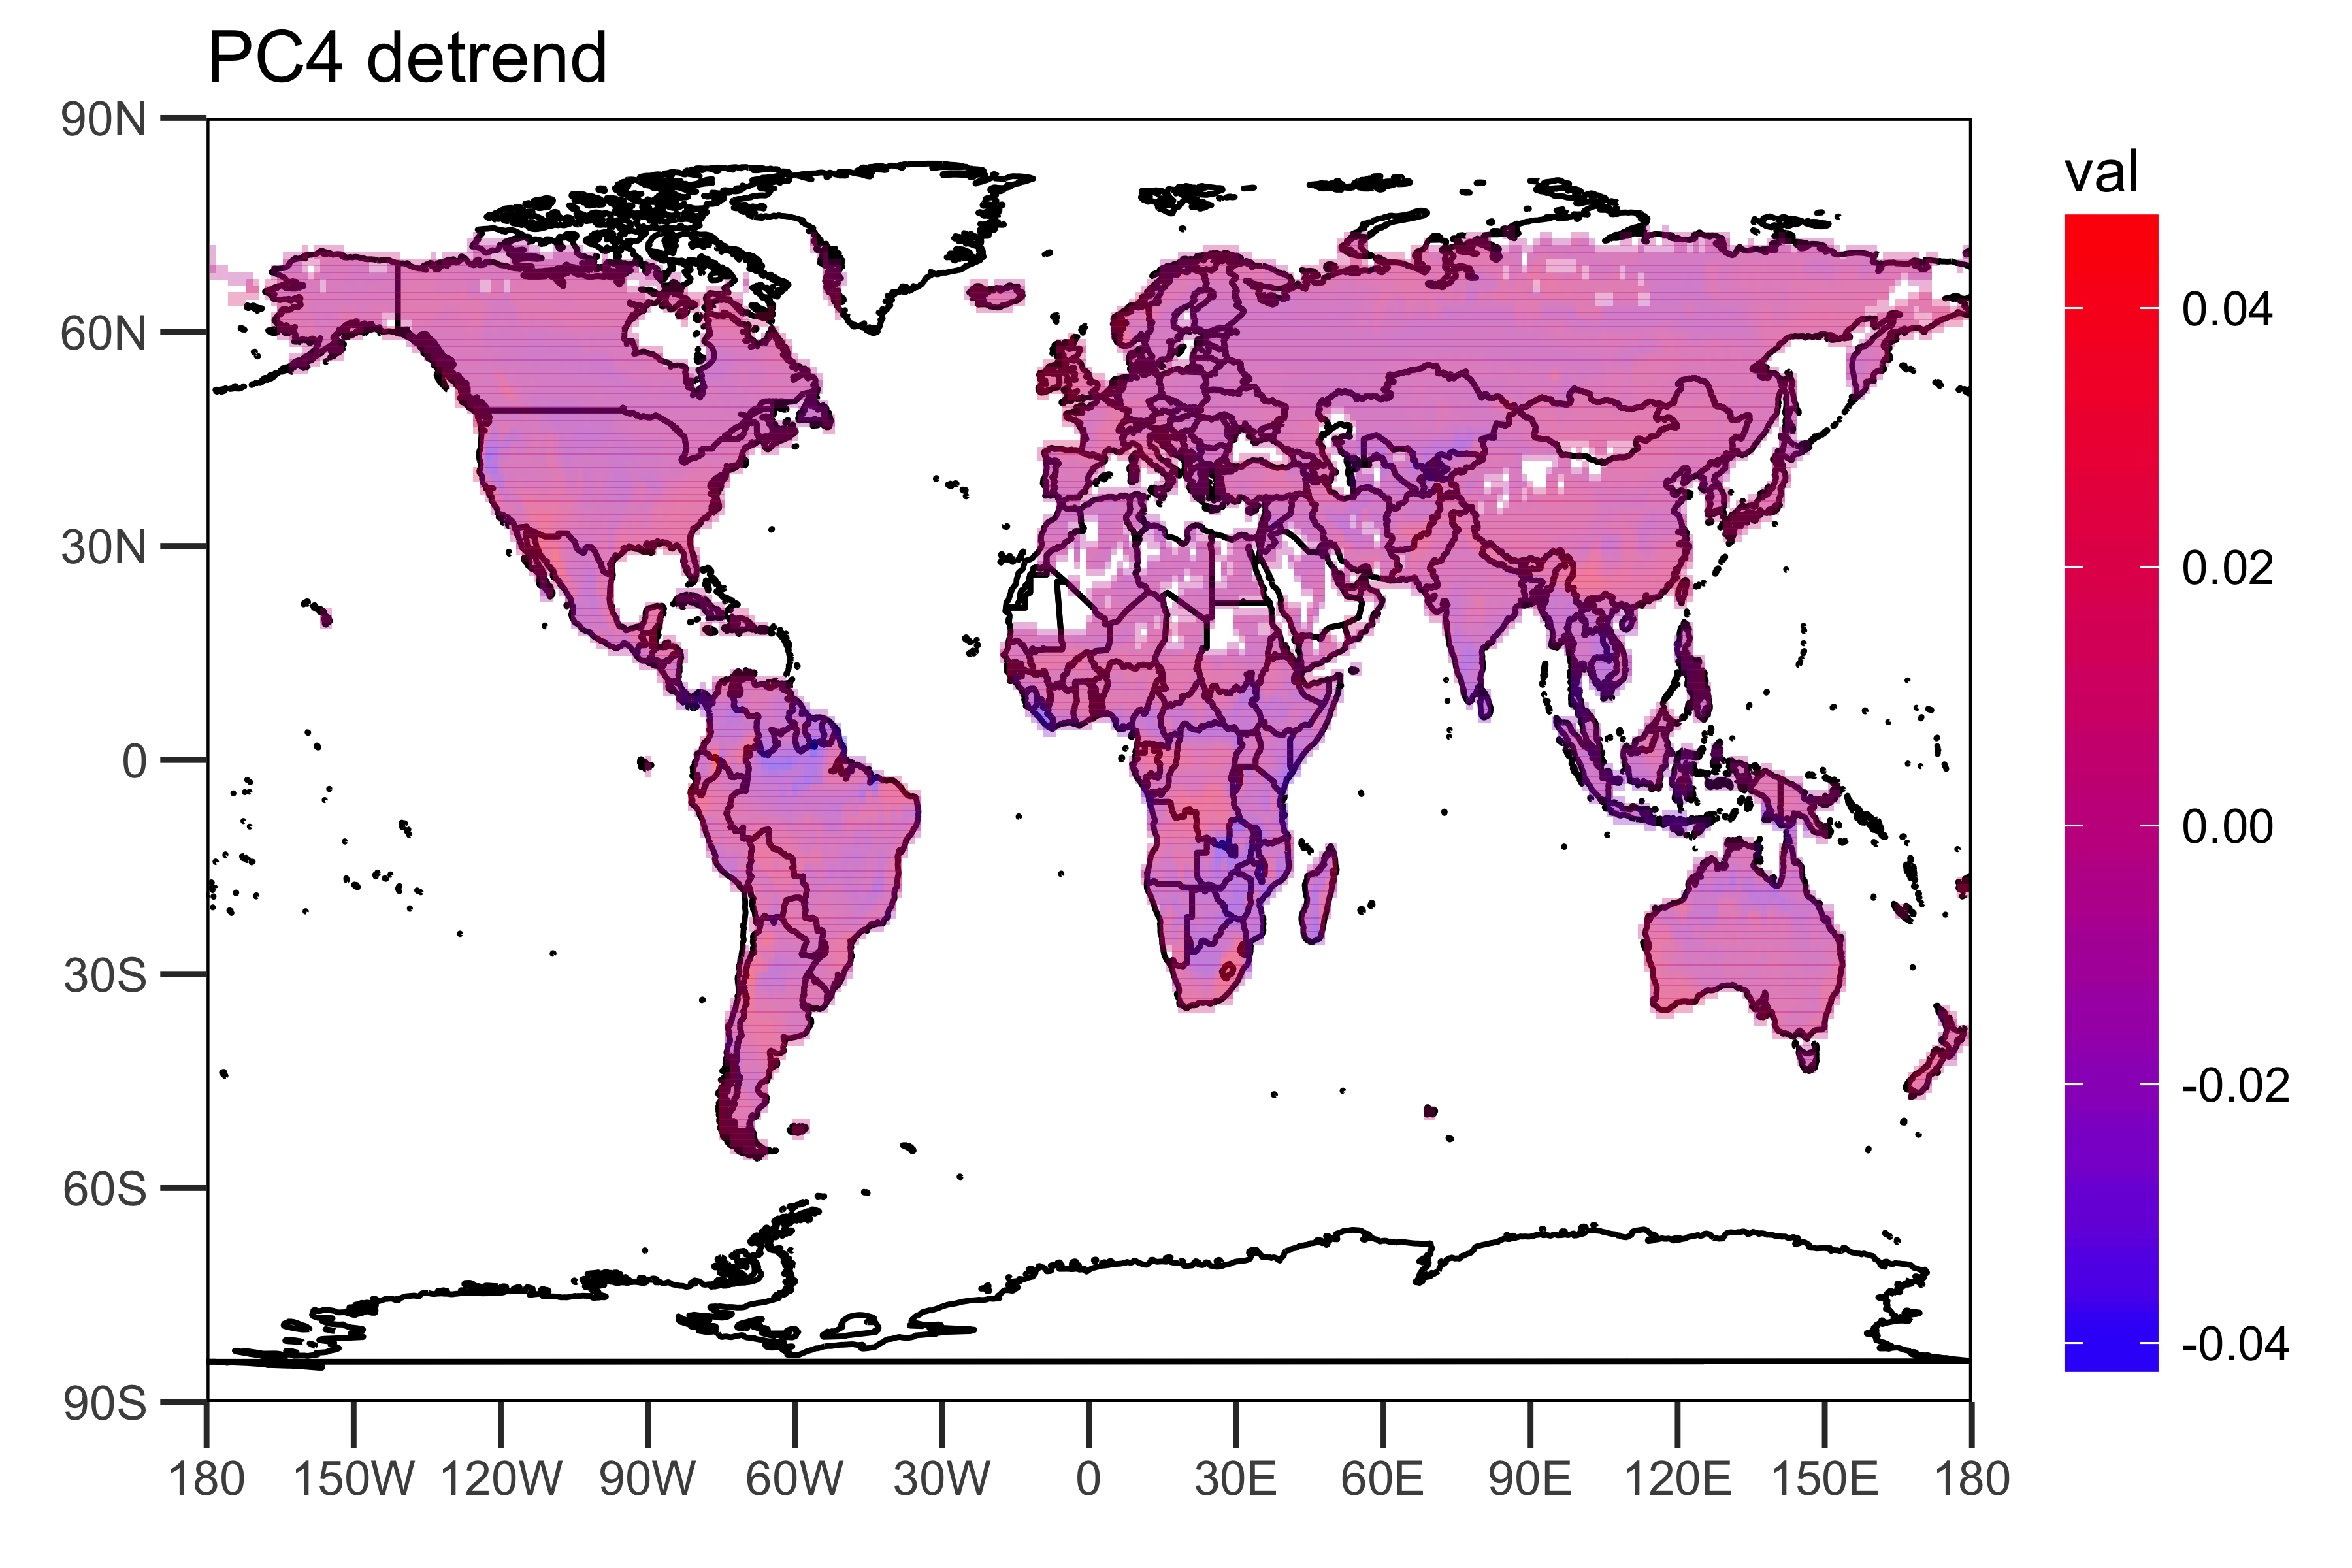
\includegraphics[width=0.45\linewidth]{../img/loading_PC4_de}}\label{fig:pc4}
	\caption{Spatial Pattern of PC 1}
\end{figure}

\subsection{Temporal Pattern}
Temporal pattern explains the dominant temporal variation of time series in the all locations, and it is represented by principal components (PCs, a number of time series) of PCA.  We can confirm the detrend first three PC are stationary in Figure~\ref{fig:pc-tsde}, and the first PC has widest range of oscillation(black) and ranges of oscillation get smaller (Blue is the second PC, and red is the third.)
\begin{figure}
	\centering
%	\subfloat[Raw Data]{\includegraphics[width=0.7\linewidth]{../img/PC-ts}}\label{fig:ts1}
	\subfloat[Detrened Data]{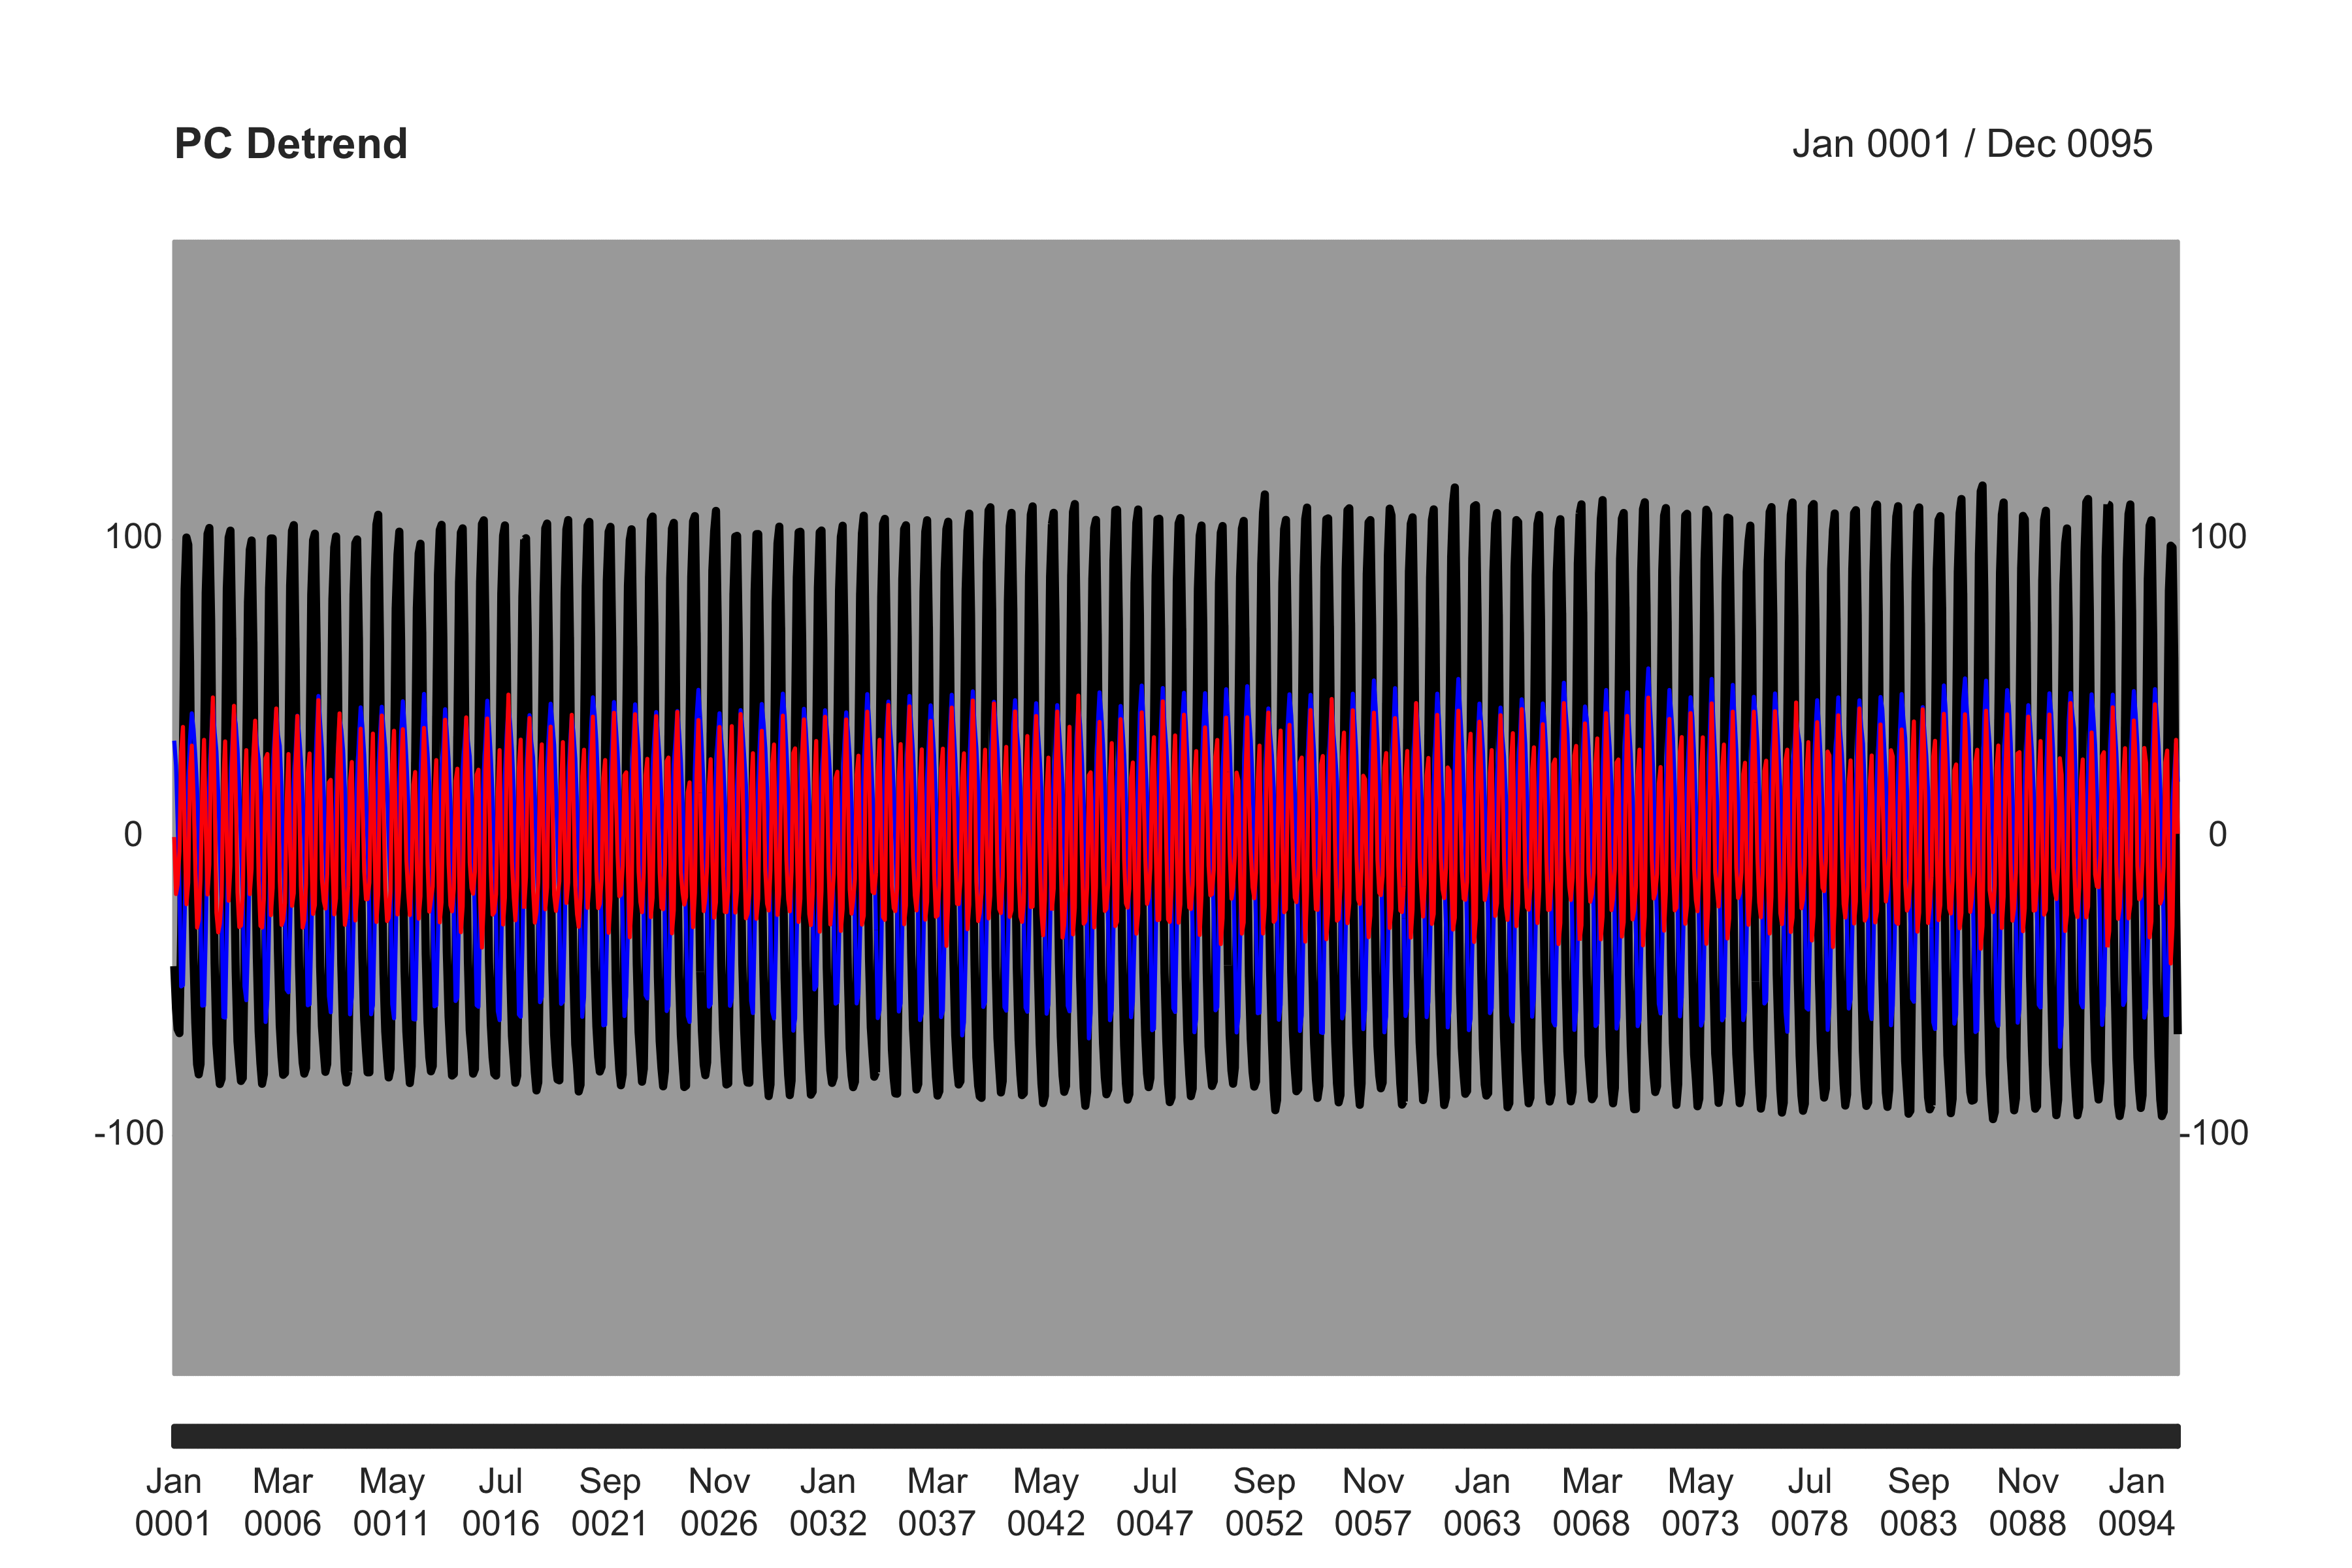
\includegraphics[width=0.7\linewidth]{../img/PC-ts_de}}\label{fig:ts2}
	\caption{PC temporal patterns}
	\label{fig:pc-tsde}
\end{figure}

We have found the PCs have seasonality through ACF in Figure~\ref{fig:pcadeacf}. PC1 and PC2 have annual seasonality, PC3 and PC4 have semi-annual, and PC5 and PC6 have quarterly seasonality, which get supported by periodograms, Figure~\ref{fig:pcaperiodogram}. It has positive and negative sides, which makes sense because the dataset has covered both north and south hemispheres. Additionally, PC1 and PC2 seems to have similar structures behind as well as PC3 and PC4 and PC5 and PC6 via the Cross-Covariance Functions in Figure~\ref{fig:pcadpeccf}. Since those have the obvious seasonality, we conduct spectral analysis on PC 1.


\paragraph{Spectral Analysis}
We model the first principal component (PC1) which has annual seasonality as:
\begin{align}
X_t &= A\cos(2\pi\frac{1}{12}t) + B\sin(2\pi\frac{1}{12}t)  \\ 
&= R\sin(2\pi\frac{1}{12} + \varphi)\\
\gamma(h) &= \sigma^2\cos(2\pi\frac{1}{12}h) 
\end{align}
where $R^2 = A^2 + B^2, \varphi = \arctan(\frac{A}{B})$.


Here is our fitted model:
\begin{align}
\hat{X}_t & = -32.652 \cos(2\pi\frac{1}{12}t) -97.1938 \sin(2\pi\frac{1}{12}t) \\
&= 102.5319\sin(2\pi\frac{1}{12}t + \frac{\pi}{10})\\
\hat{\gamma}(h) &= 13.93^2\cos(2\pi\frac{1}{12}h) 
\end{align}

This model can explains 96\% variances (Adjusted $R^2$ is 0.9644). The PC 2 can be fitted by 
\begin{equation}
\hat{X}_t = 48.96085\sin(2\pi\frac{1}{12}-\frac{2\pi}{5} ),\; \hat{\sigma}^2 = 8.17
\end{equation}
which is shifted and smaller oscillations with respect to PC1 model. 

\paragraph{} Interestingly, we find another cycles from the residuals of the PC1 model.  If we allow to add more cyclic variables, we could end up:
\begin{align}
X_t &= c_1\cos(2\pi\frac{1}{12}t) + c_2\sin(2\pi\frac{1}{12}t) + c_3\cos(2\pi\frac{1}{6}t) + c_4\sin(2\pi\frac{1}{6}t) \notag\\
&+ c_5\cos(2\pi\frac{1}{4}t) + c_6\cos(2\pi\frac{1}{3}t) + c_7\sin(2\pi\frac{1}{3}t)  + c_8\sin(2\pi t)
\end{align}
this model can explain 99.62\% variances. 

\appendix
\section{Simulation}
All analysis in this report was performed on a single ensemble submission to the
NCAR CMIP database. The ensemble's Project ID in the CMIP5 database is
cmip5.output1.NCAR.CCSM4.rcp45.mon.land.Lmon.r2i1p1.v20140403|esgf-data.ucar.edu.
Its version number is 20140403. To download the bash script that will download
the data for you, follow this link:
\url{https://esgf-node.llnl.gov/esg-search/wget/?distrib=false&dataset_id=cmip5.output1.NCAR.CCSM4.rcp45.mon.land.Lmon.r2i1p1.v20140403|esgf-data.ucar.edu}

.

\section{PCA}
\subsection{Tables}
\begin{table}[ht]
	\centering
	\begin{tabular}{rrrrrrr}
		\hline
		& PC1 & PC2 & PC3 & PC4 & PC5 & PC6 \\ 
		\hline
		StDev & 66.650 & 28.003 & 24.356 & 20.348 & 17.832 & 12.301 \\ 
		Prop. of Var. & 0.347 & 0.061 & 0.046 & 0.032 & 0.025 & 0.012 \\ 
		Cum. Prop.& 0.347 & 0.408 & 0.454 & 0.486 & 0.511 & 0.523 \\ 
		\hline
	\end{tabular}
	\caption{Explained Variations of PC: Raw Dataset}\label{table:rawdataprop}
\end{table}
\begin{table}[ht]
	\centering
	\begin{tabular}{rrrrrrr}
		\hline
		& PC1 & PC2 & PC3 & PC4 & PC5 & PC6 \\ 
		\hline
		StDev & 73.857 & 35.586 & 23.852 & 14.581 & 11.859 & 10.669 \\ 
		Prop. of Var. & 0.426 & 0.099 & 0.044 & 0.017 & 0.011 & 0.009 \\ 
		Cum. Prop. & 0.426 & 0.524 & 0.569 & 0.585 & 0.596 & 0.605 \\ 
		\hline
	\end{tabular}
	\caption{Explained Variations of PC: Detrendset}\label{table:detrendprop}
\end{table}
\pagebreak
\subsection{Plots}
\begin{figure}[!tbp]
	\centering
		\subfloat[PC 1]{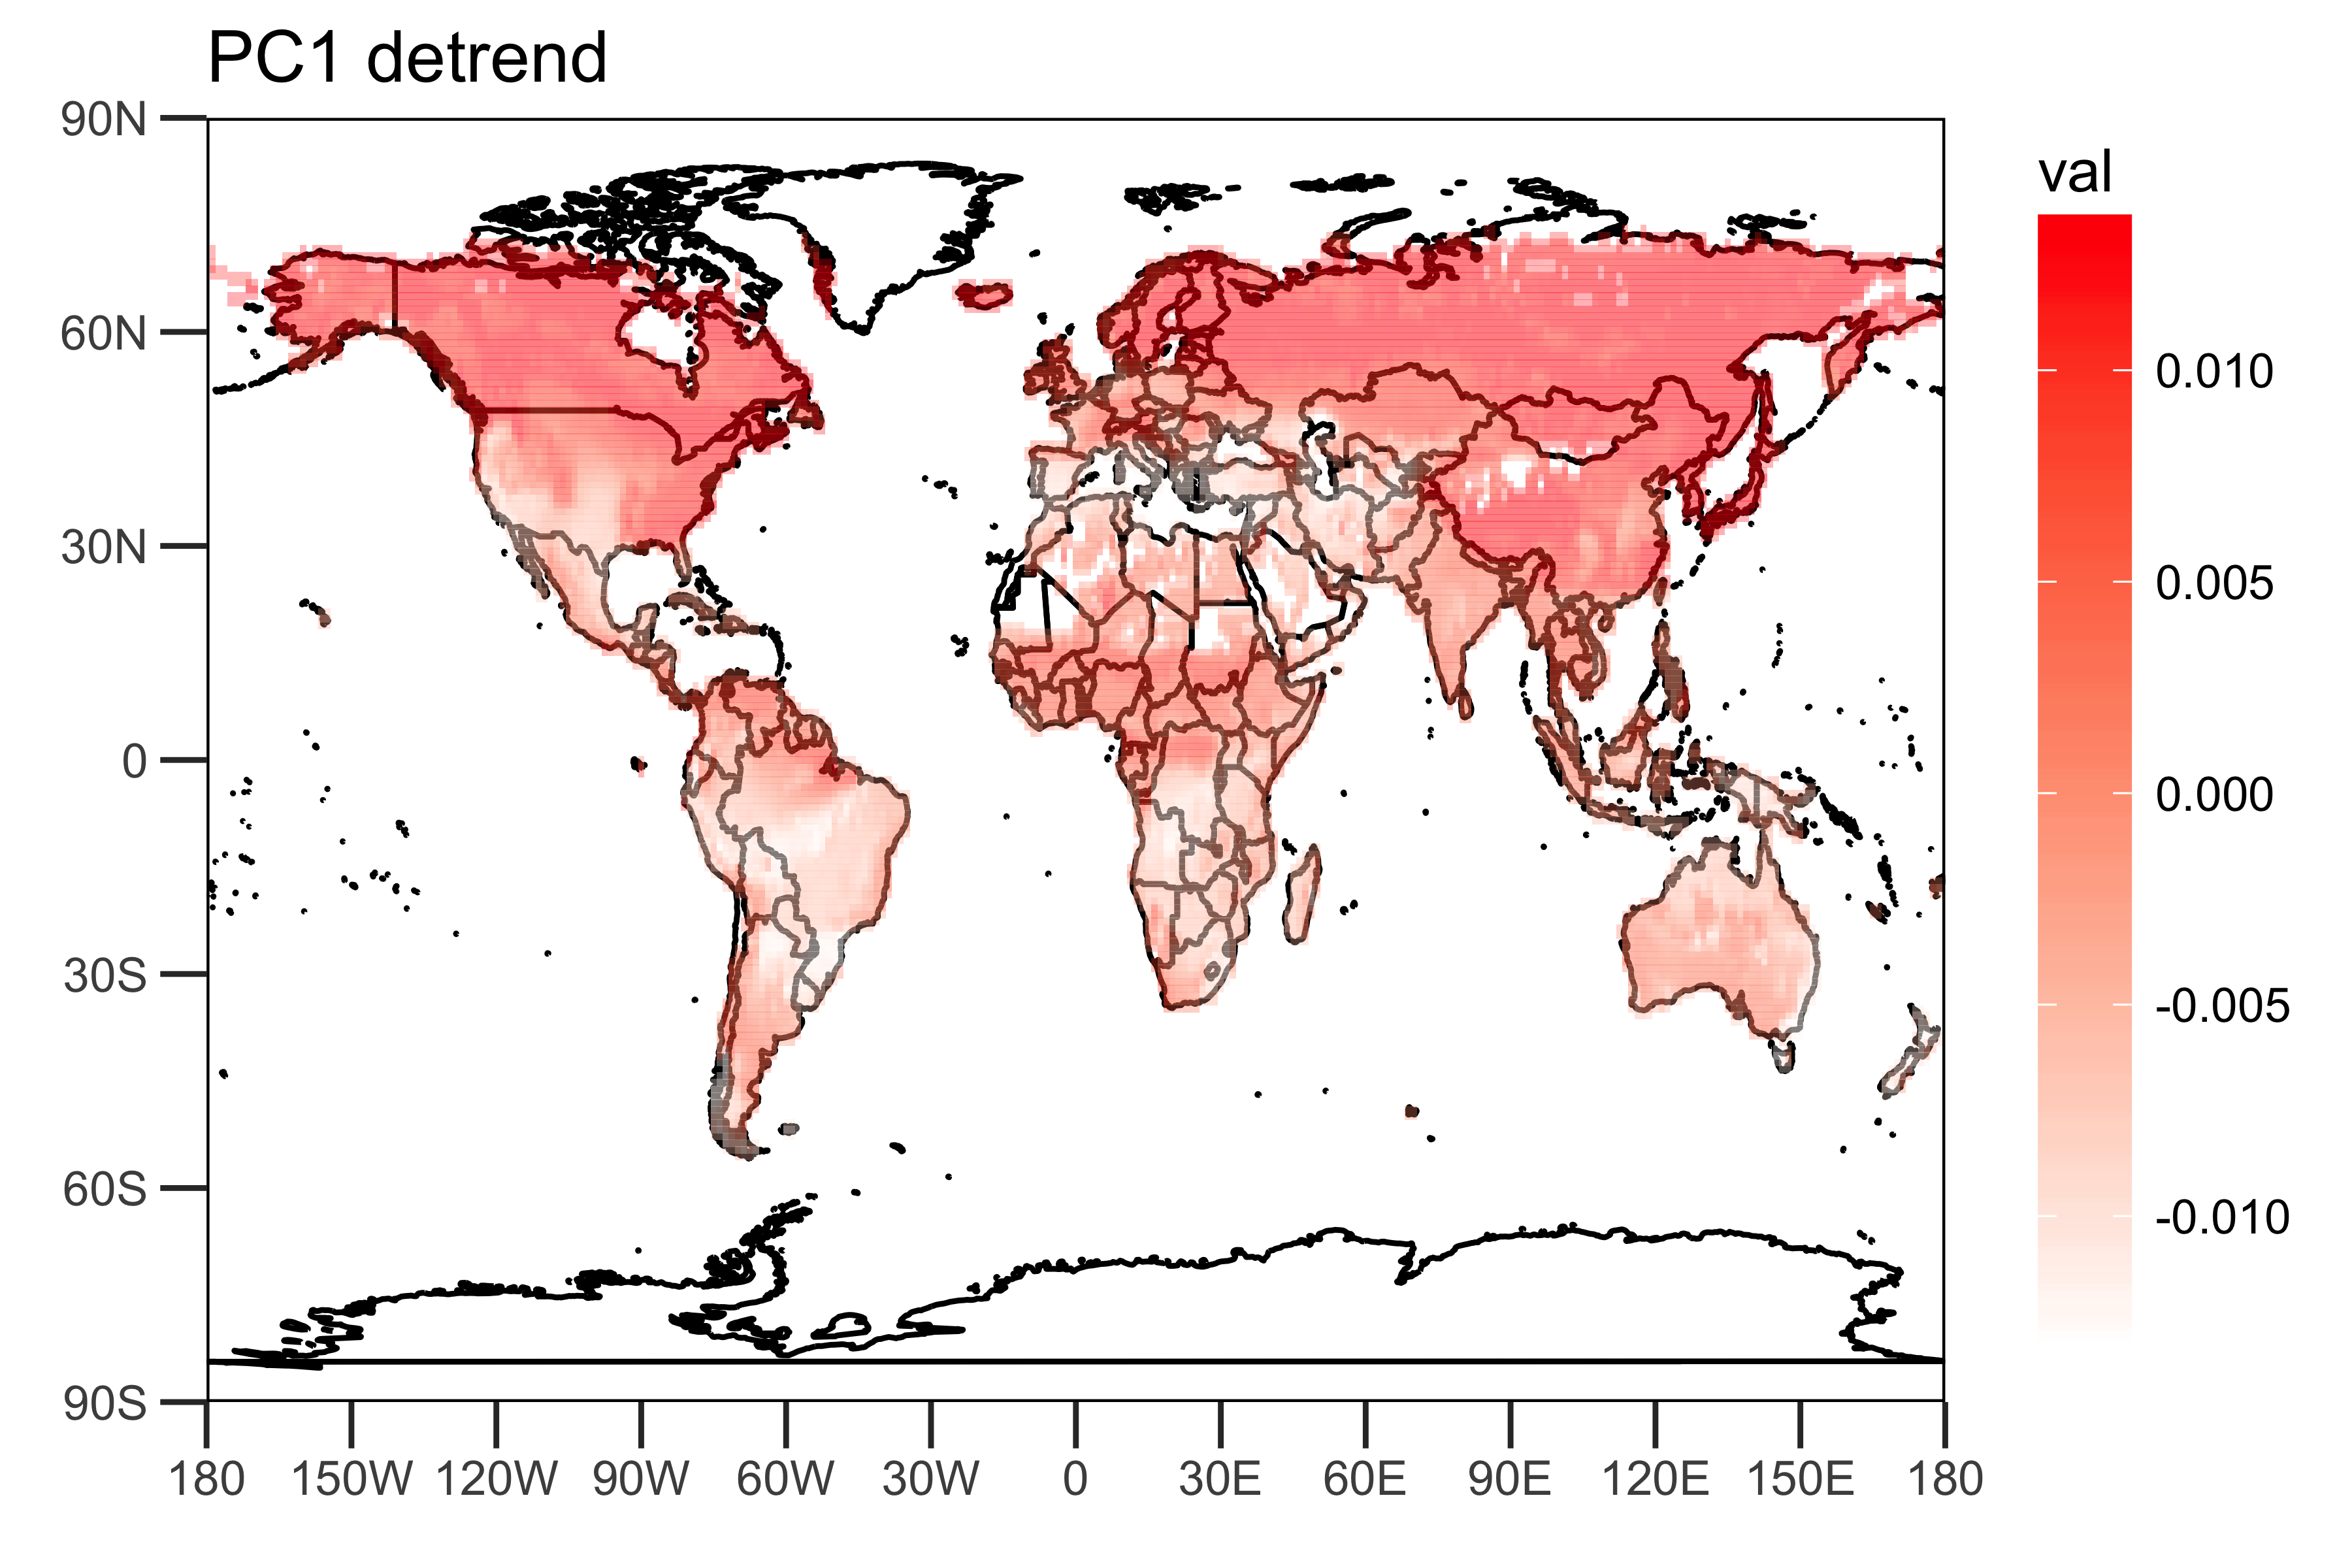
\includegraphics[width=0.45\linewidth]{../img/loading_PC1_de}}\label{fig:pc1}
		\hfill
		\subfloat[PC 2]{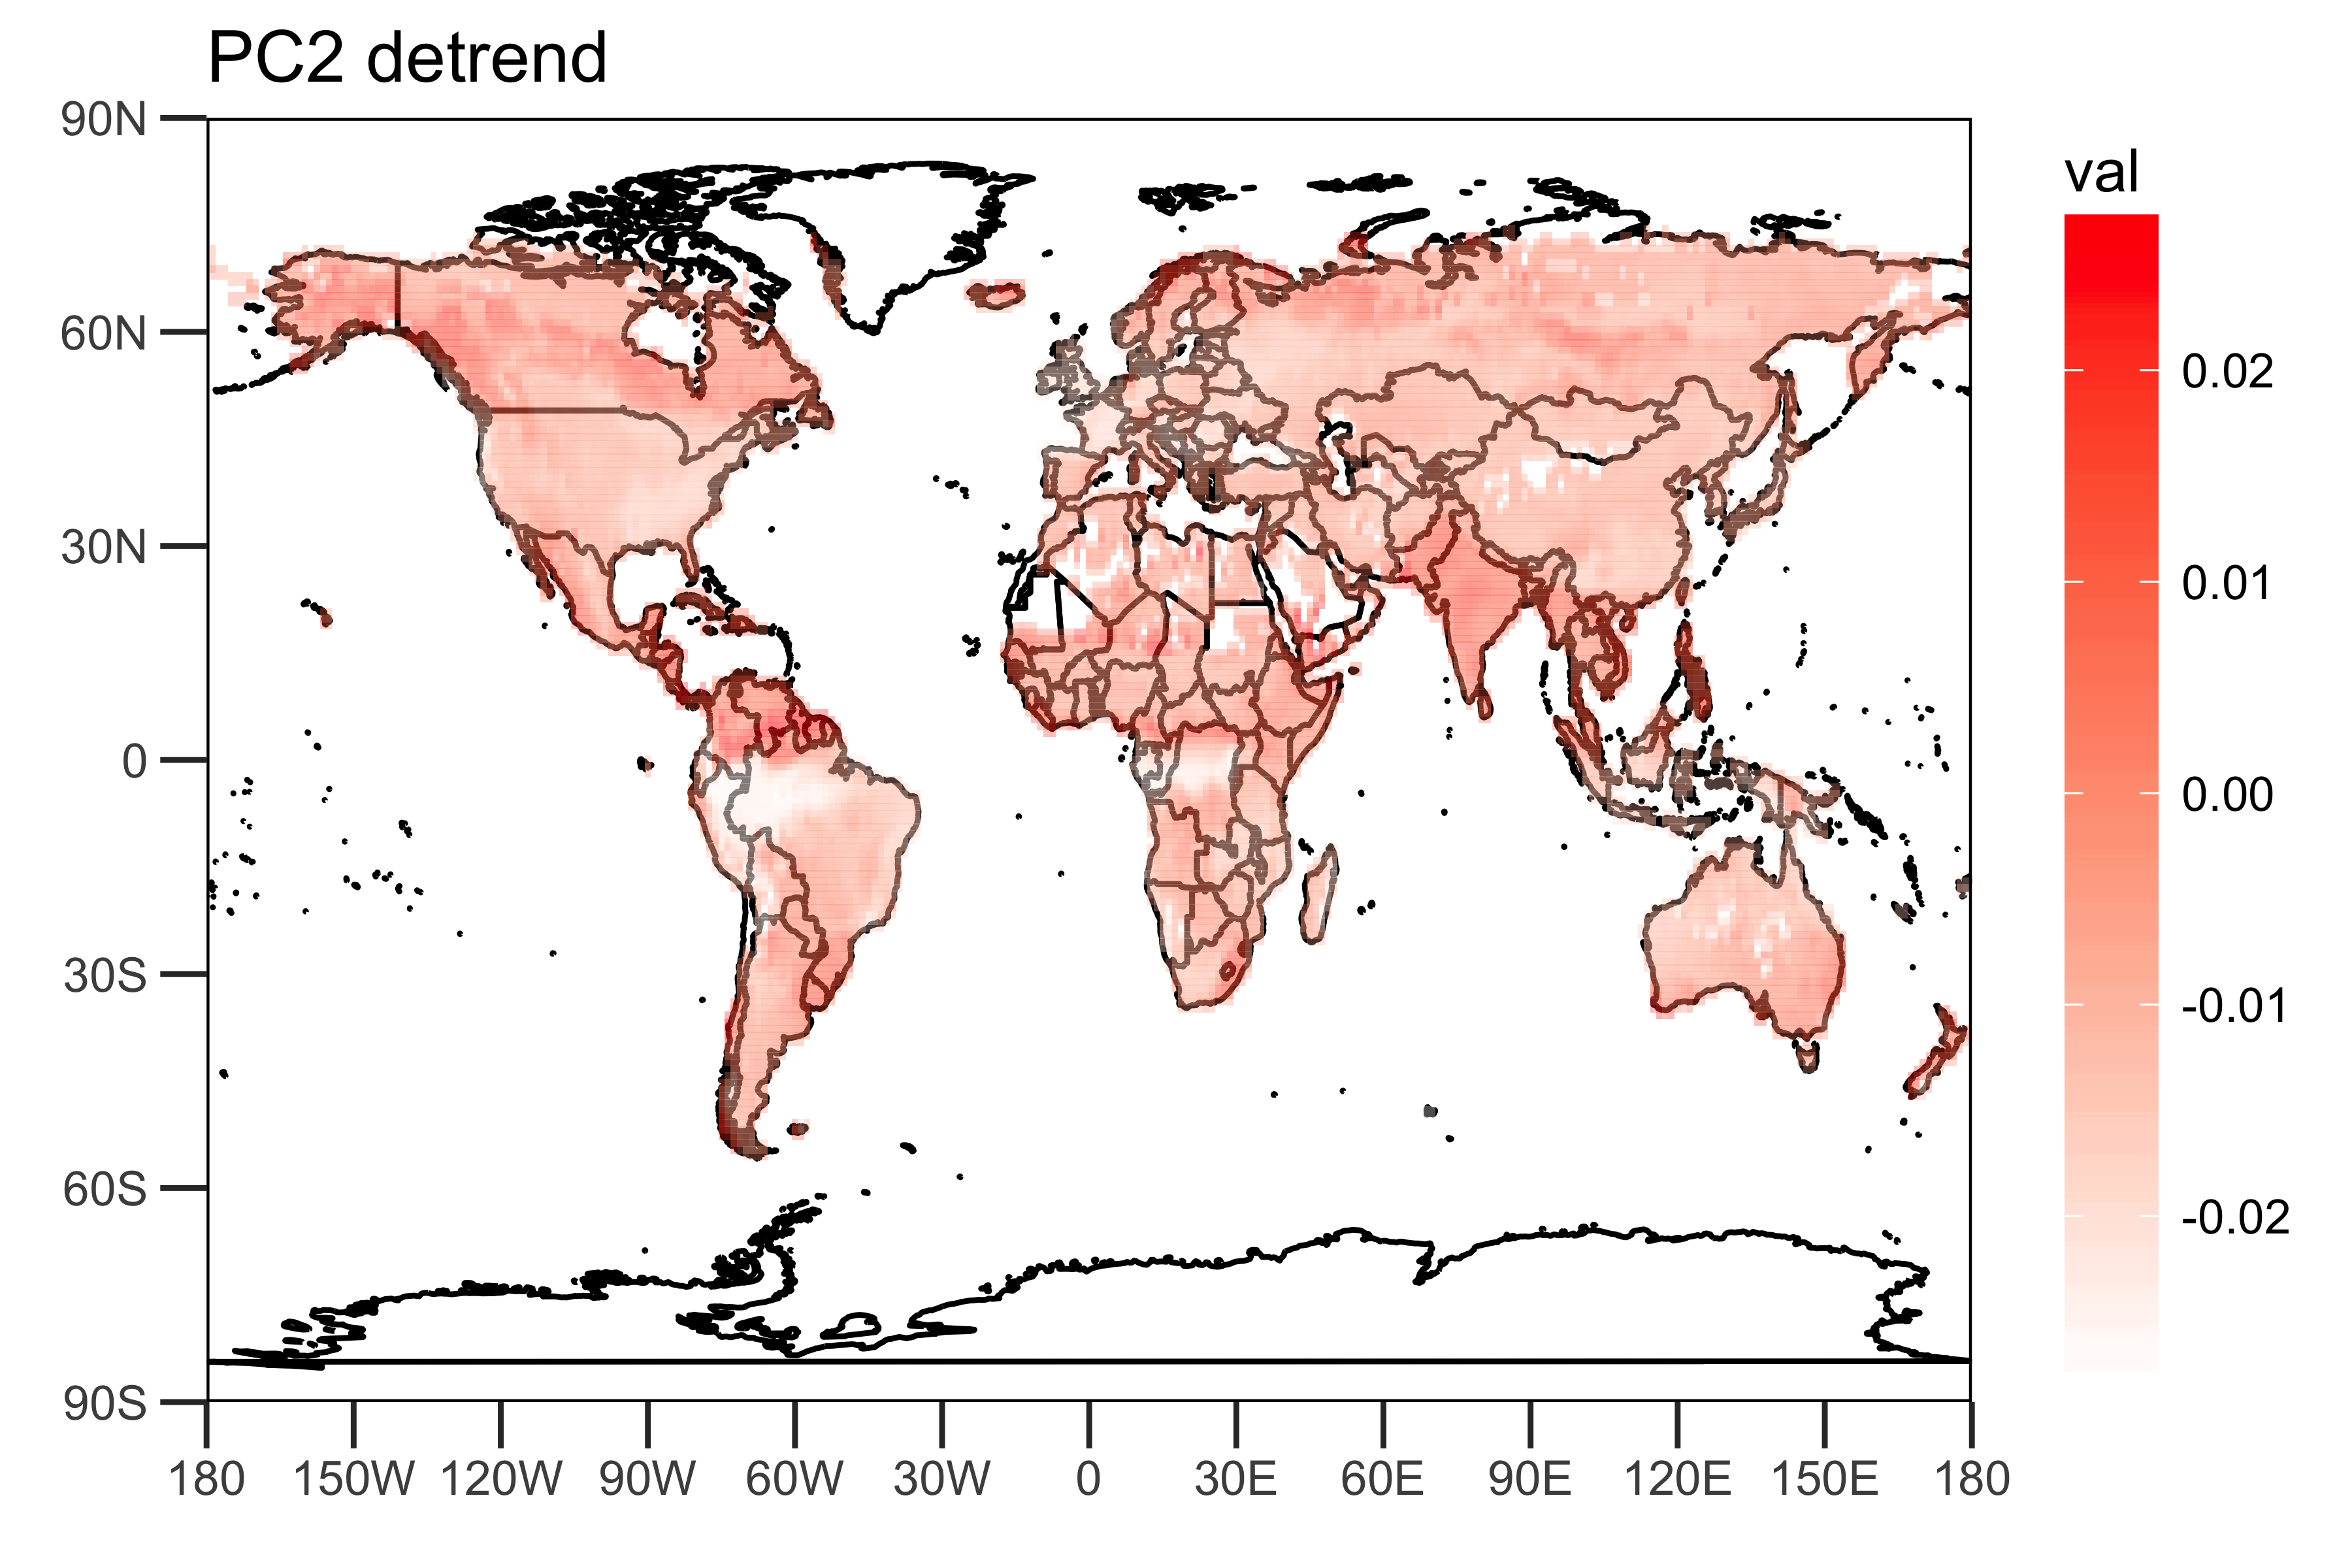
\includegraphics[width=0.45\linewidth]{../img/loading_PC2_de}}\label{fig:pc2}
		\subfloat[PC 3]{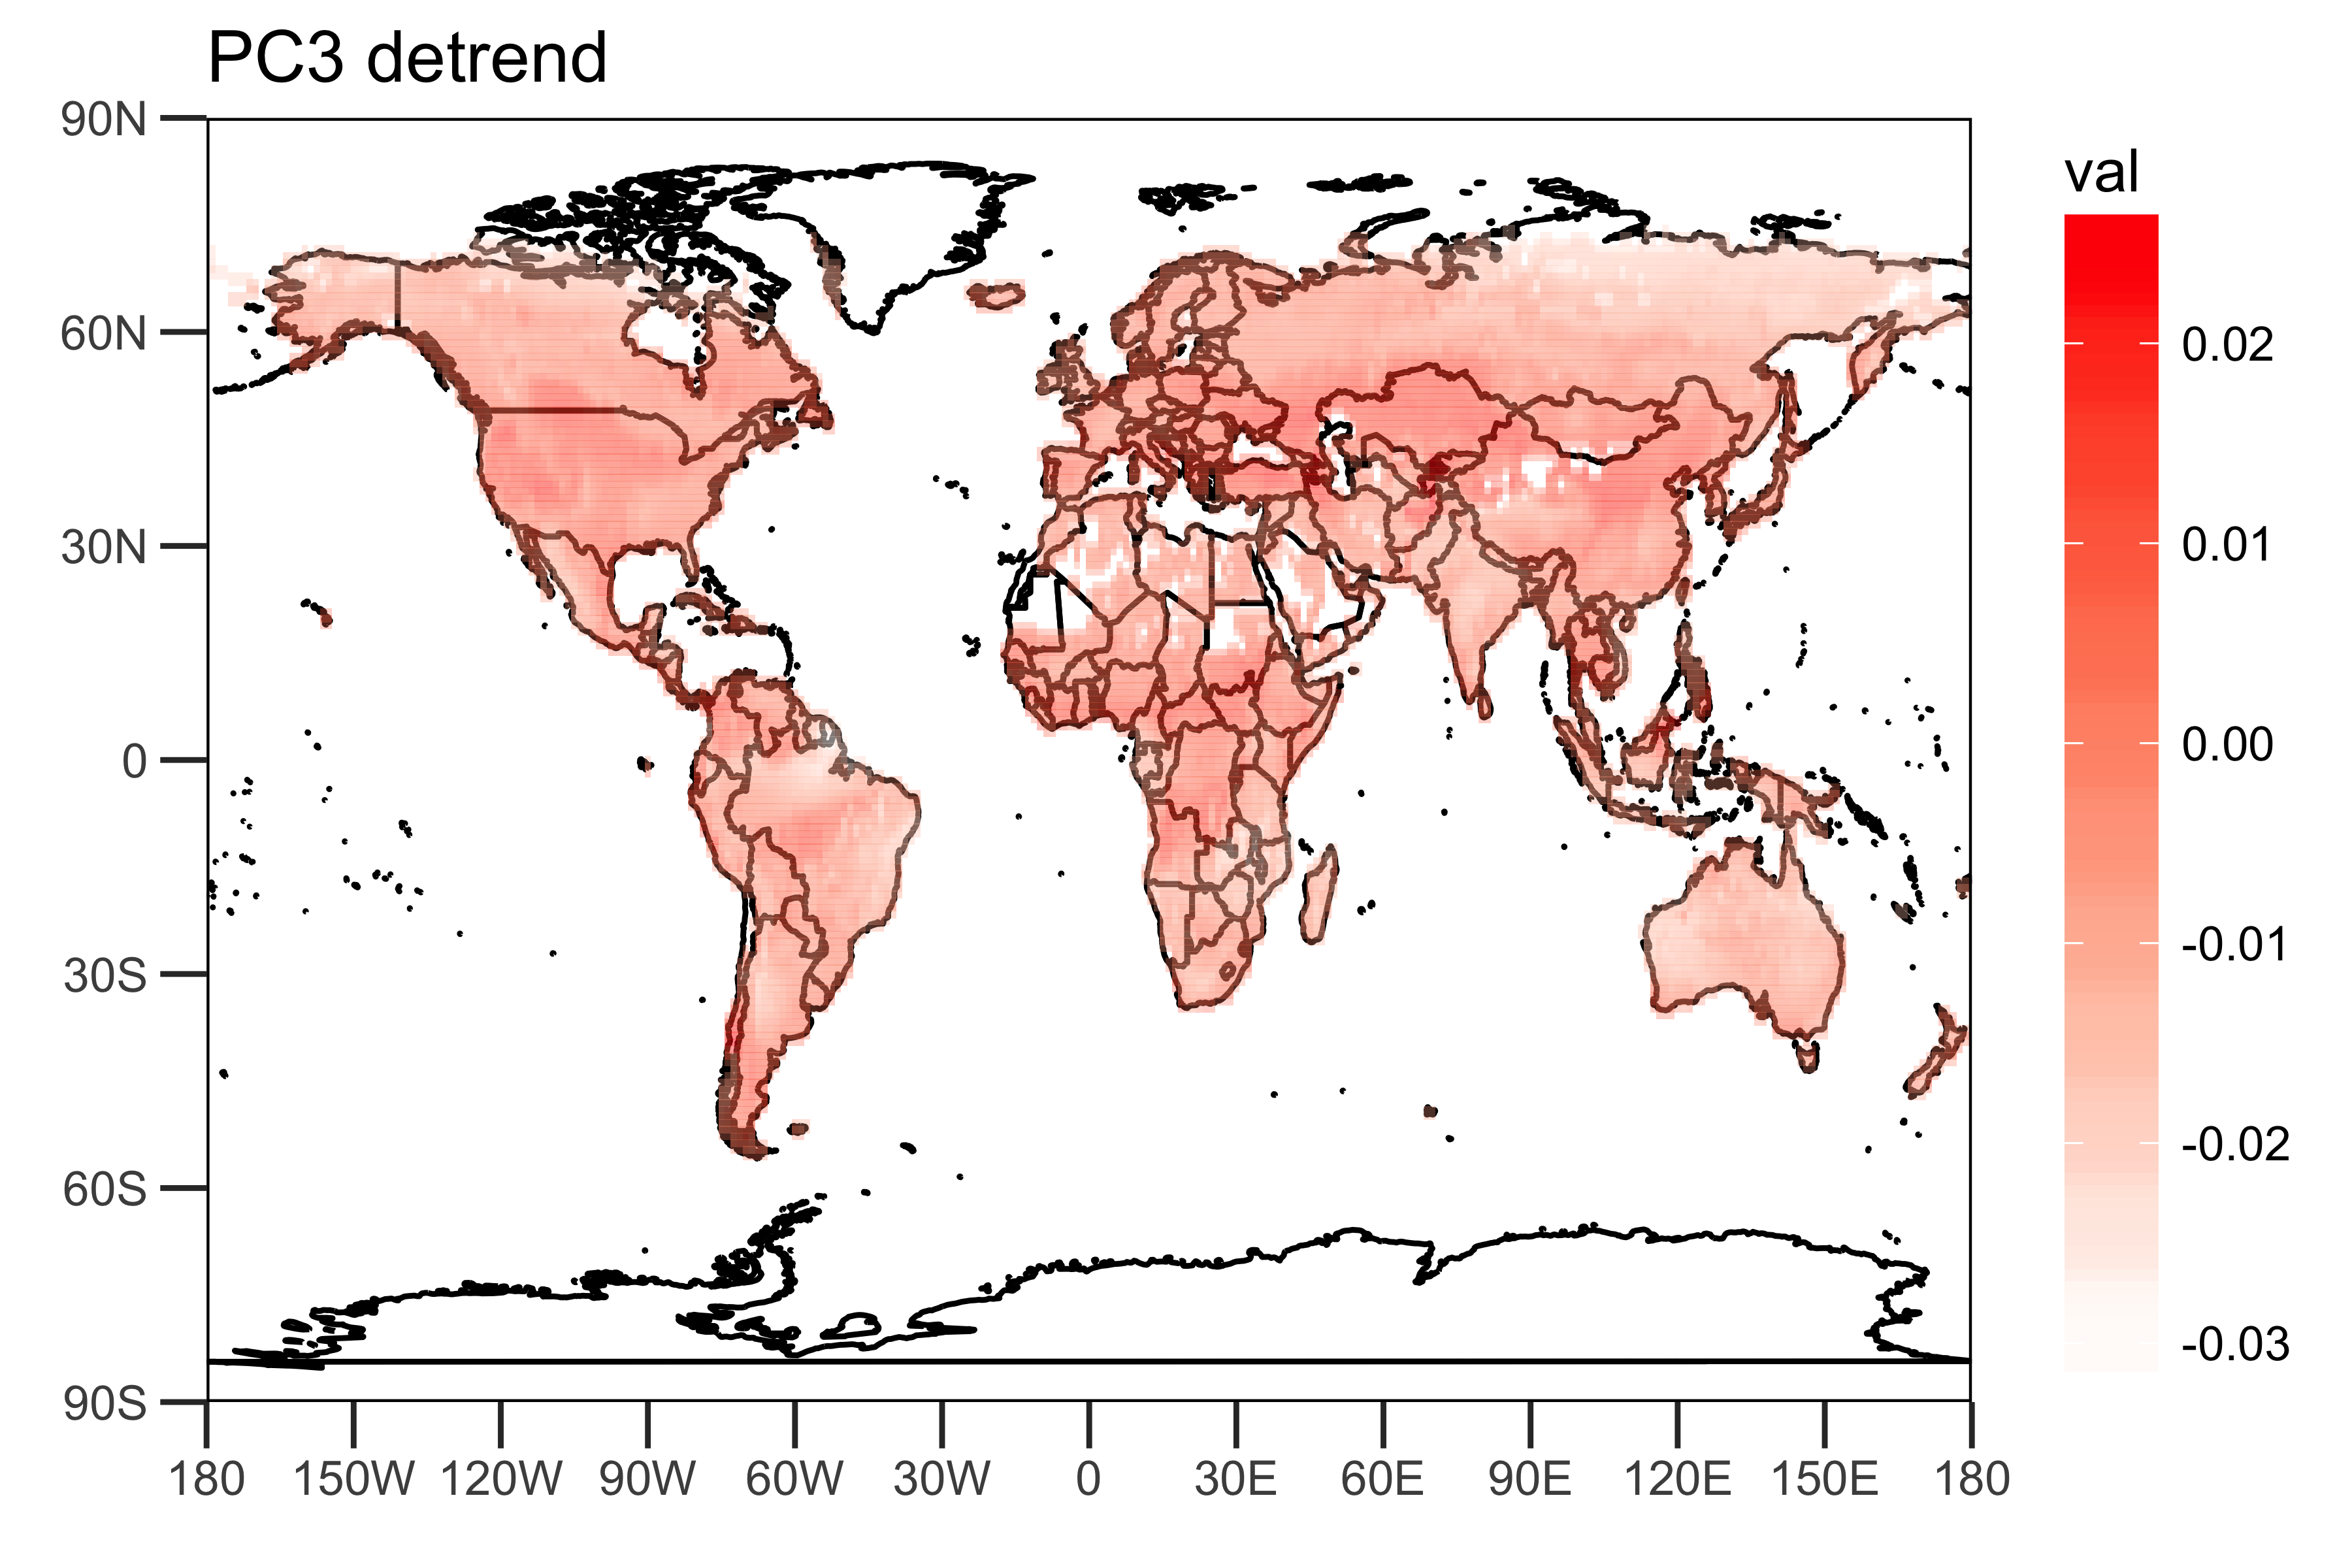
\includegraphics[width=0.45\linewidth]{../img/loading_PC3_de}}\label{fig:pc3}
		\hfill
		\subfloat[PC 4]{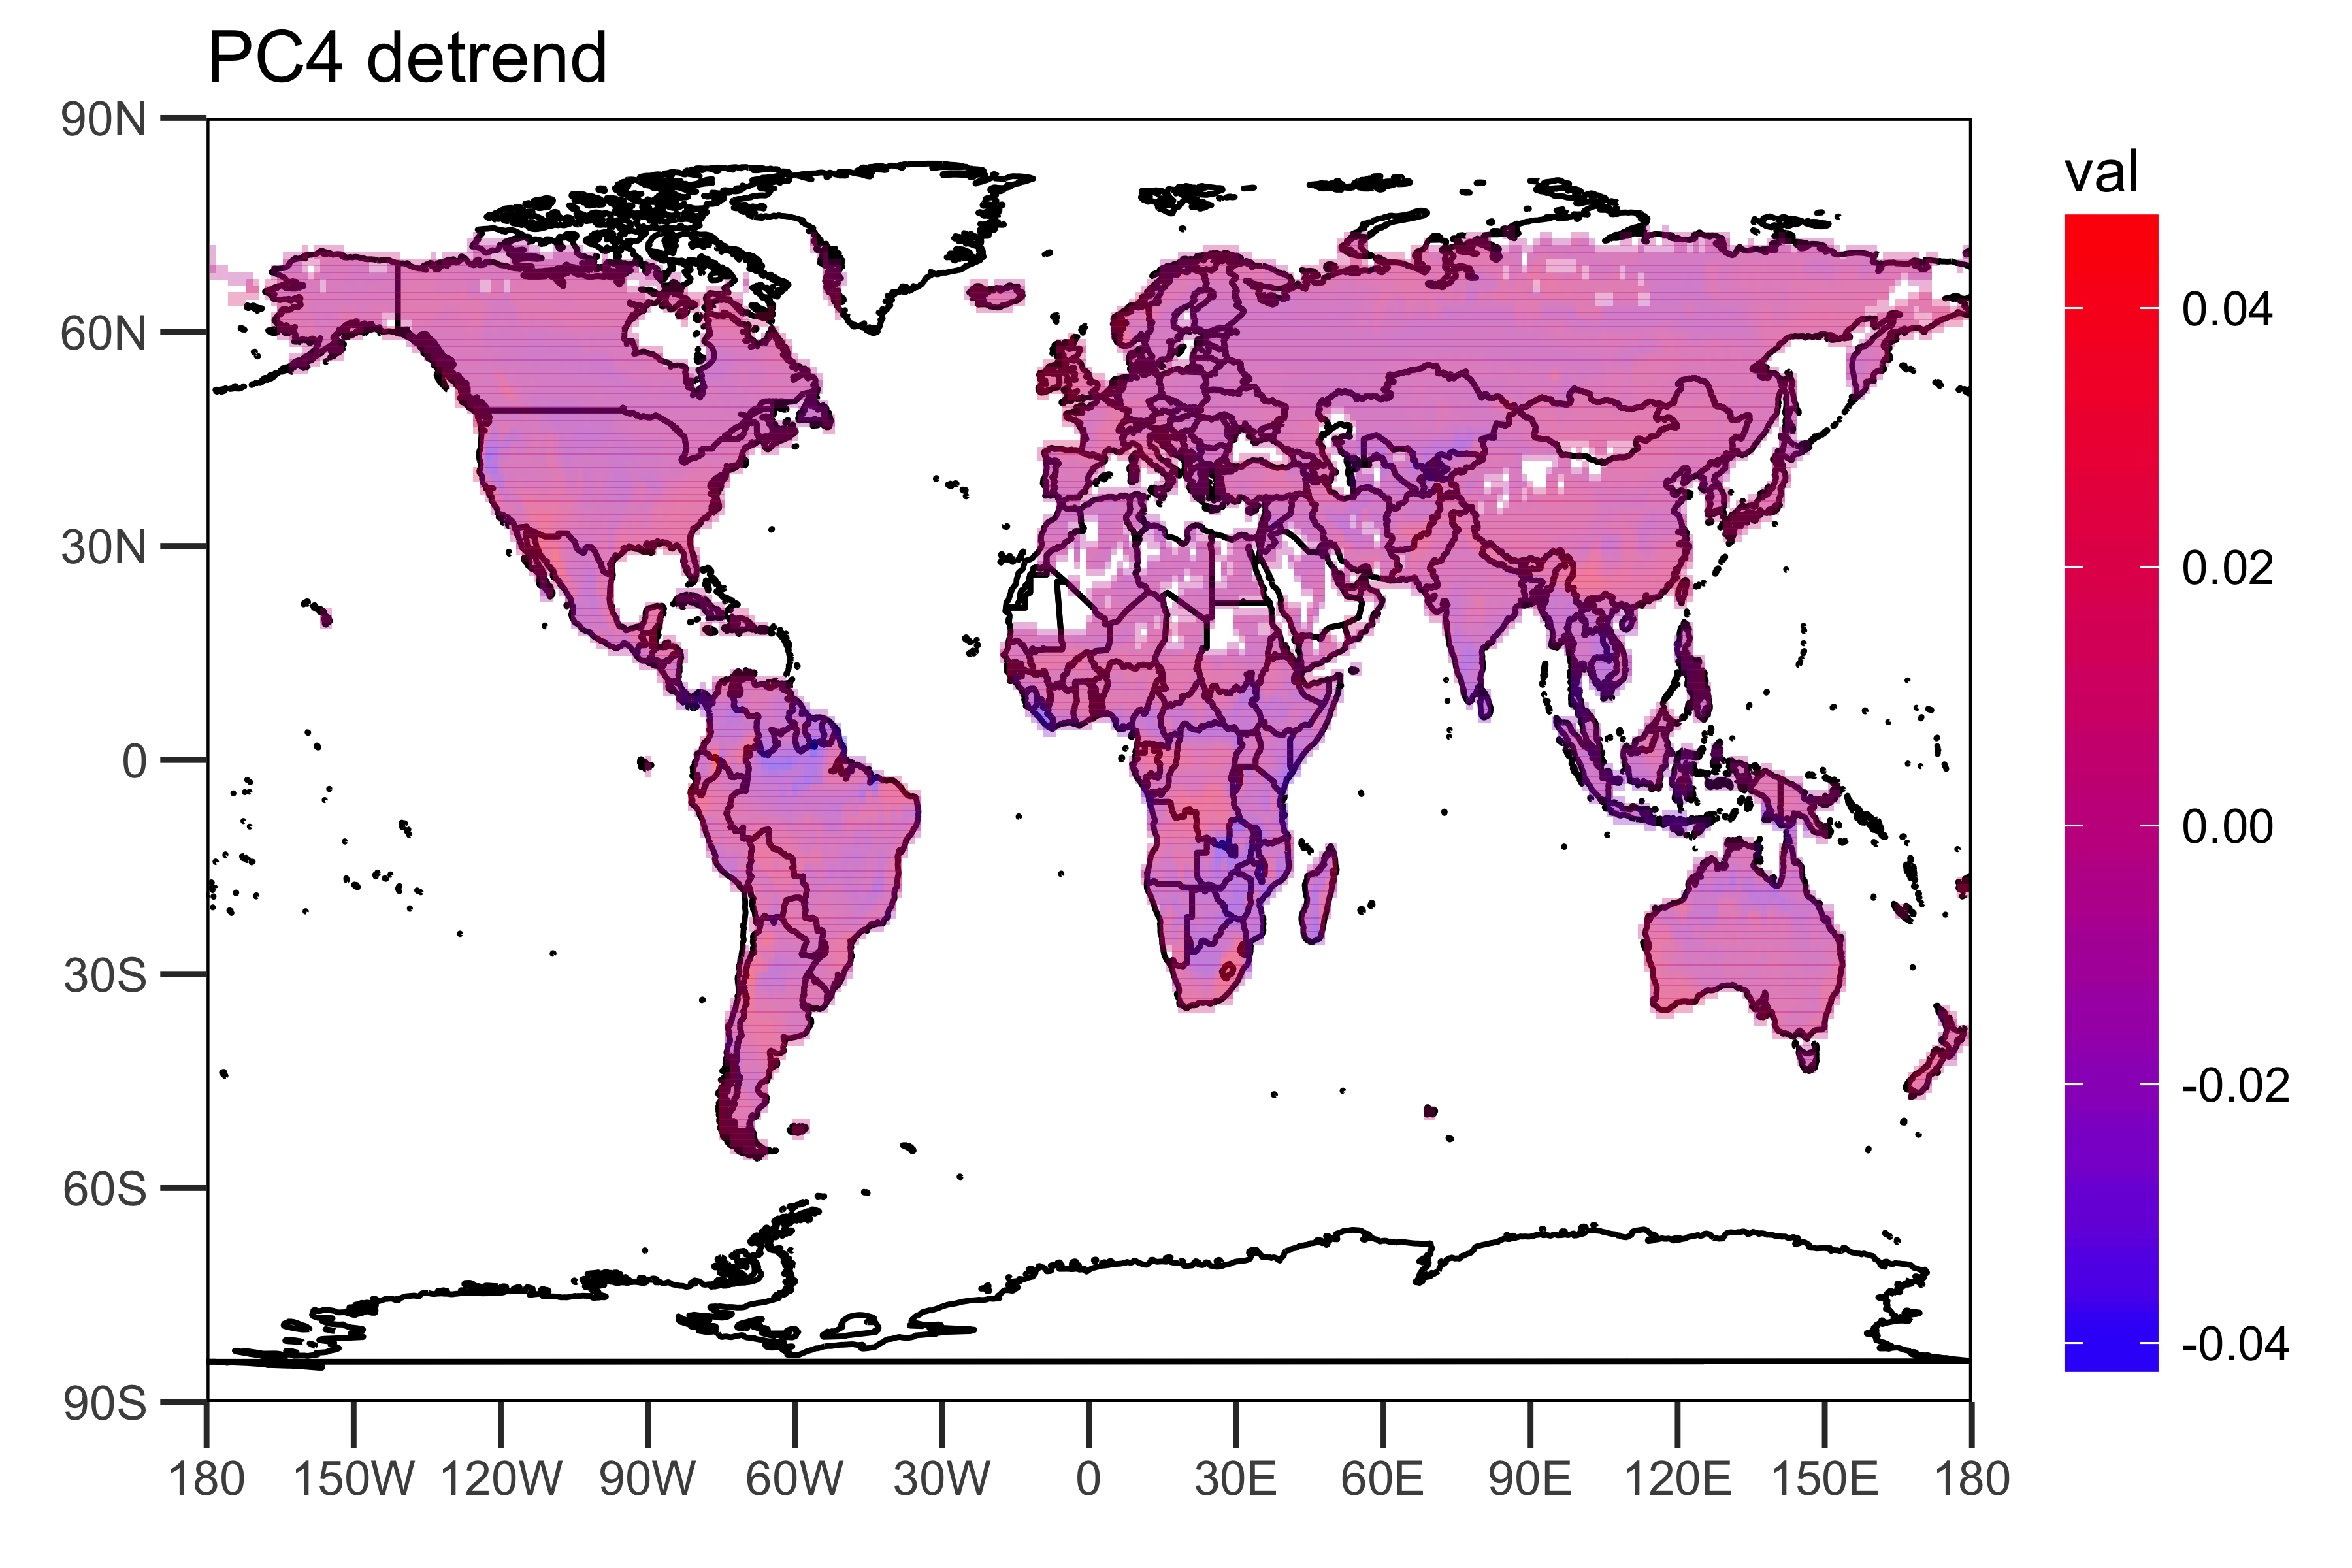
\includegraphics[width=0.45\linewidth]{../img/loading_PC4_de}}\label{fig:pc4}
		\subfloat[PC 5]{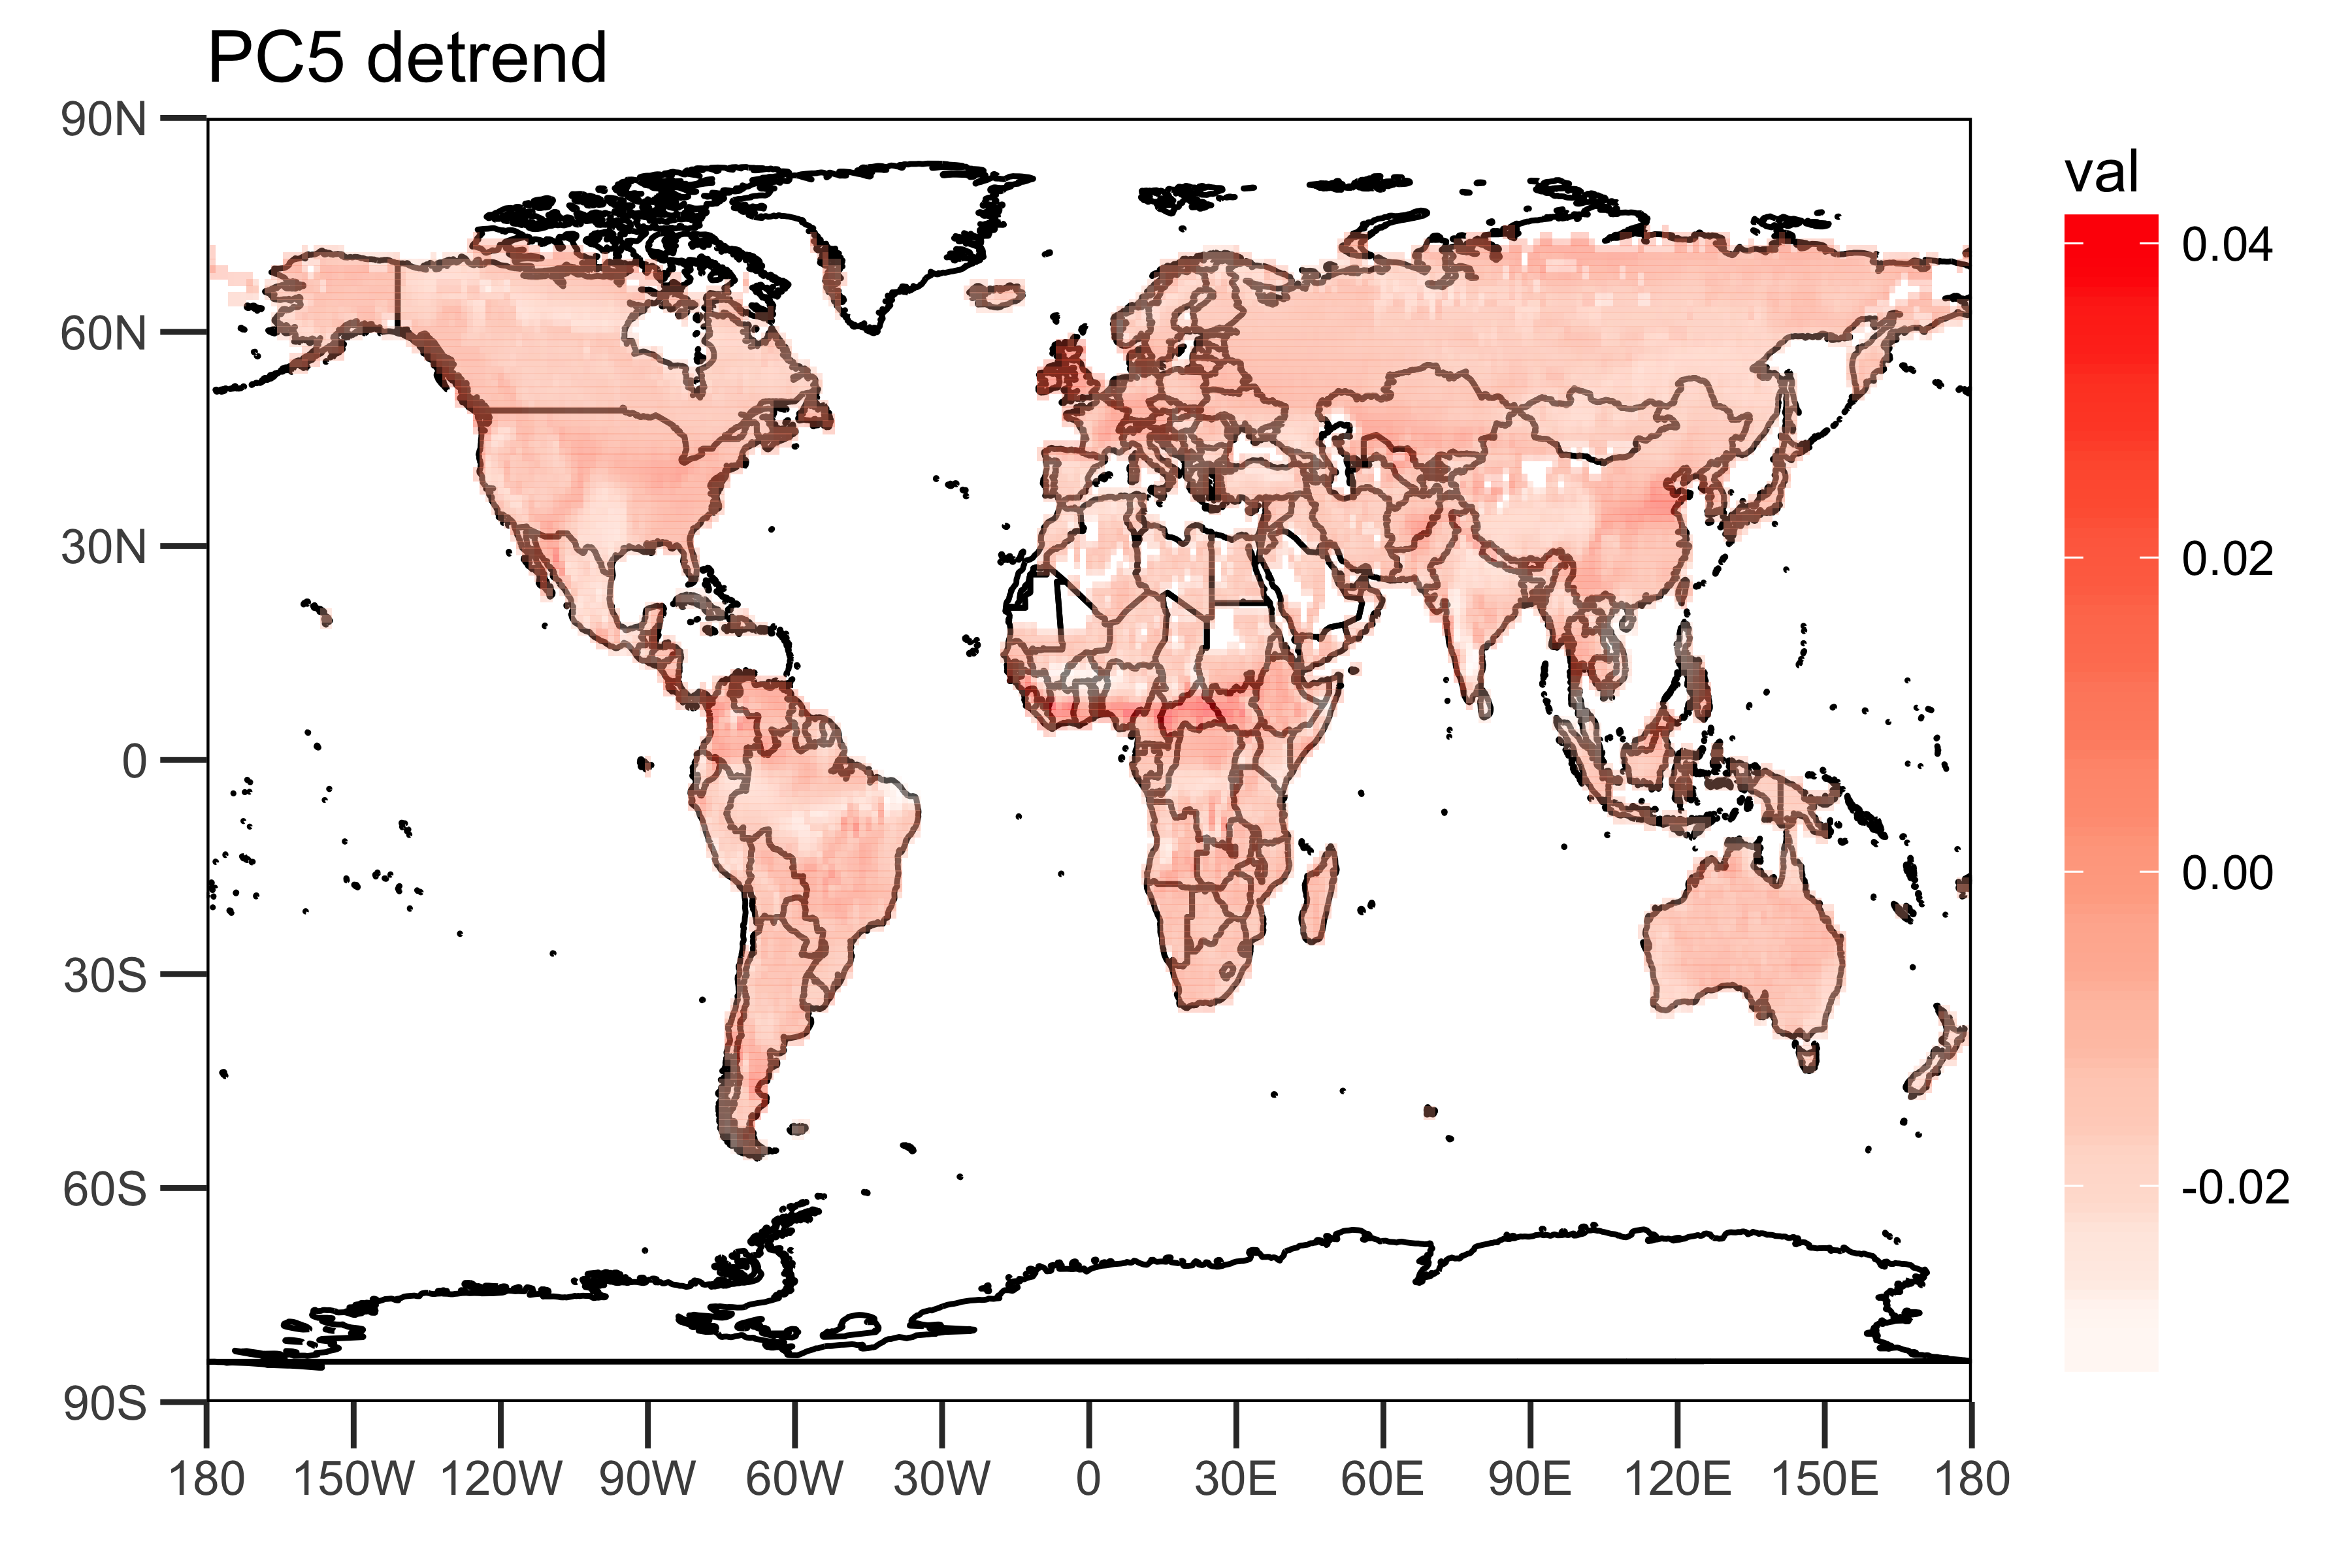
\includegraphics[width=0.45\linewidth]{../img/loading_PC5_de}}\label{fig:pc5}
		\hfill
		\subfloat[PC 6]{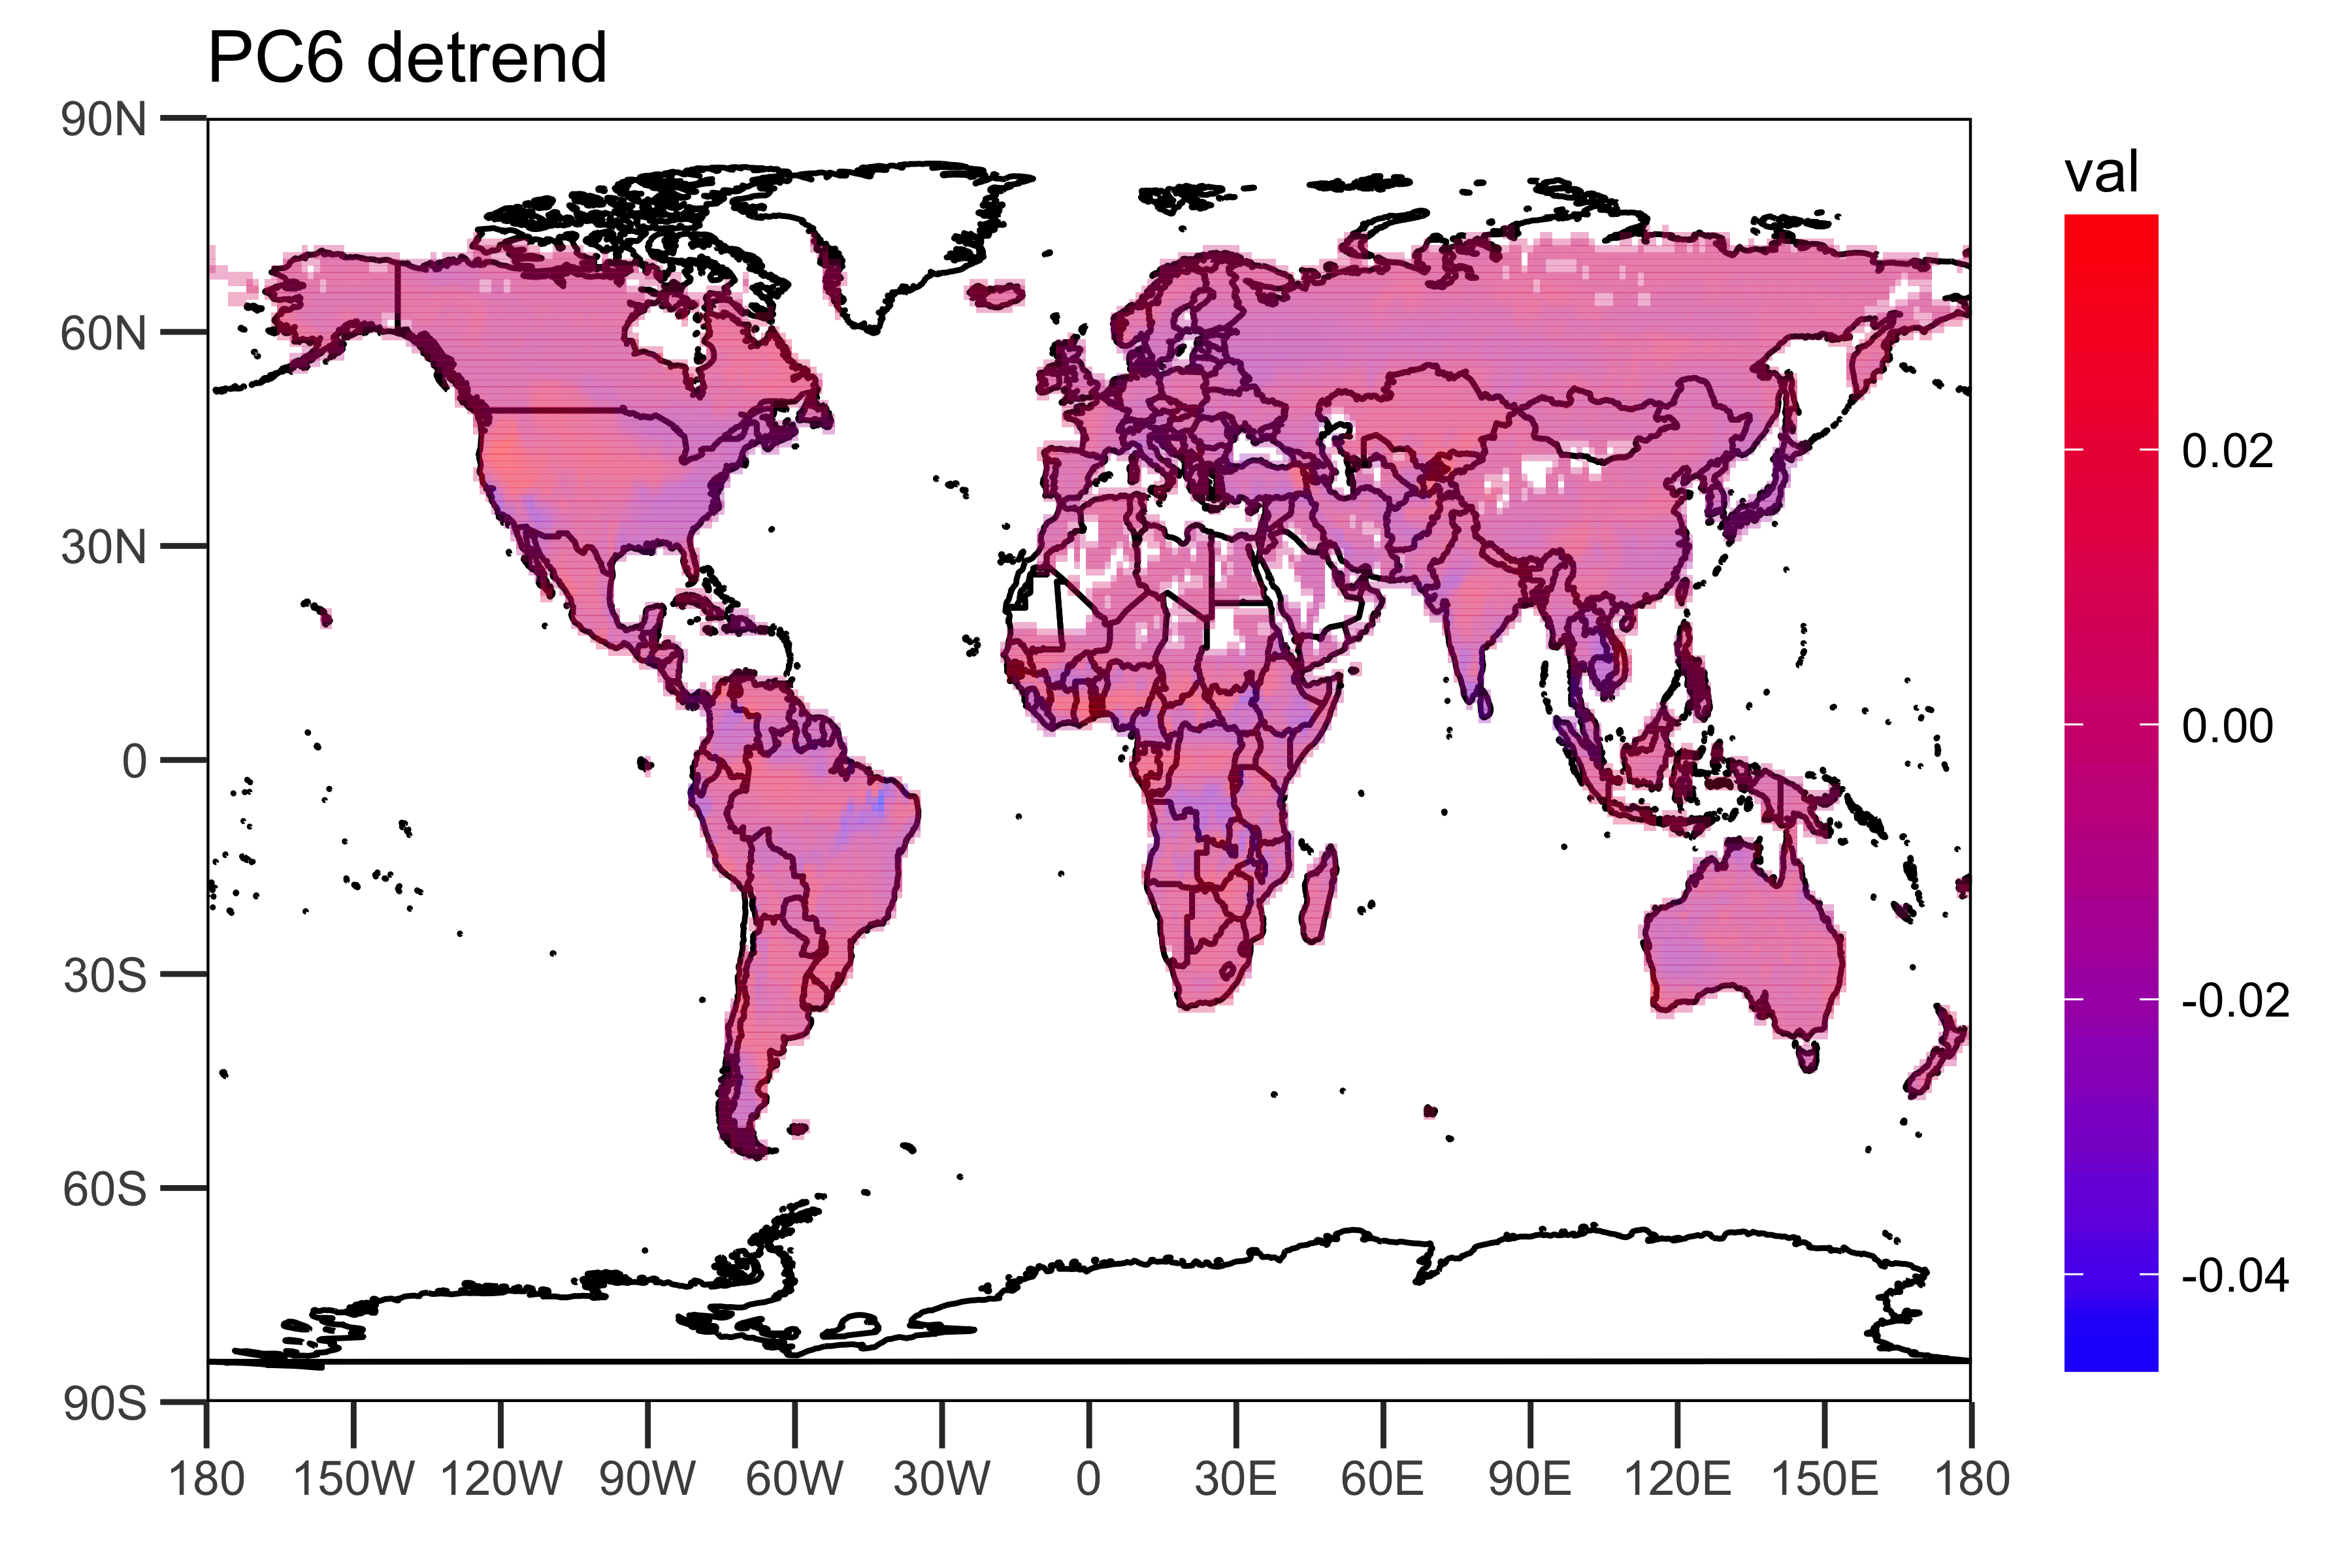
\includegraphics[width=0.45\linewidth]{../img/loading_PC6_de}}\label{fig:pc6}
	\caption{Spatial Patterns}\label{fig:spatialpatter6}
\end{figure}

\begin{figure}[!tbp]
	\centering
	\subfloat[Raw Data]{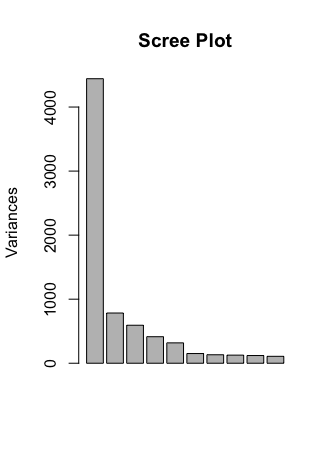
\includegraphics[height=0.4\textheight]{../img/Scree_plot1}\label{fig:screeplotf1}}
	\hfill
	\subfloat[Detrended Data]{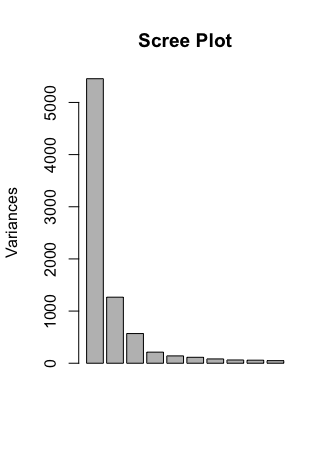
\includegraphics[height=0.4\textheight]{../img/Scree_plot2}\label{fig:screeplotf2}}
	\caption{Scree Plots}\label{fig:screeplot}
\end{figure}

\begin{figure}
	\centering
	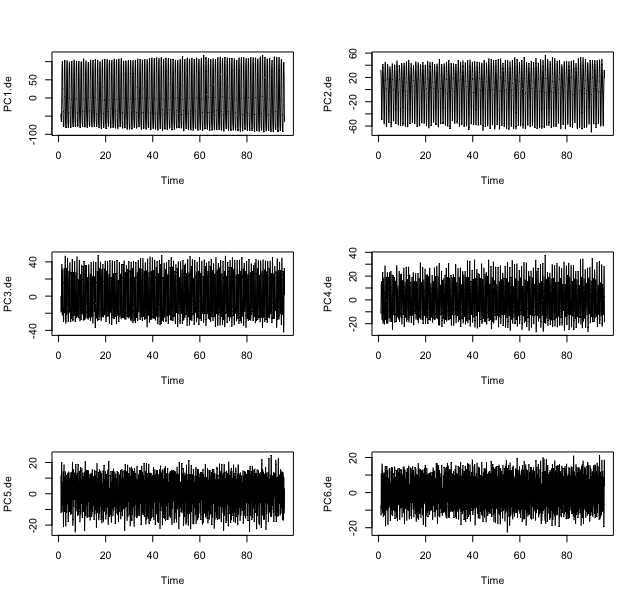
\includegraphics[width=0.7\linewidth]{../img/PCA_ts}
	\caption{Time Series Plots}
	\label{fig:pcats}
\end{figure}

\begin{figure}
	\centering
	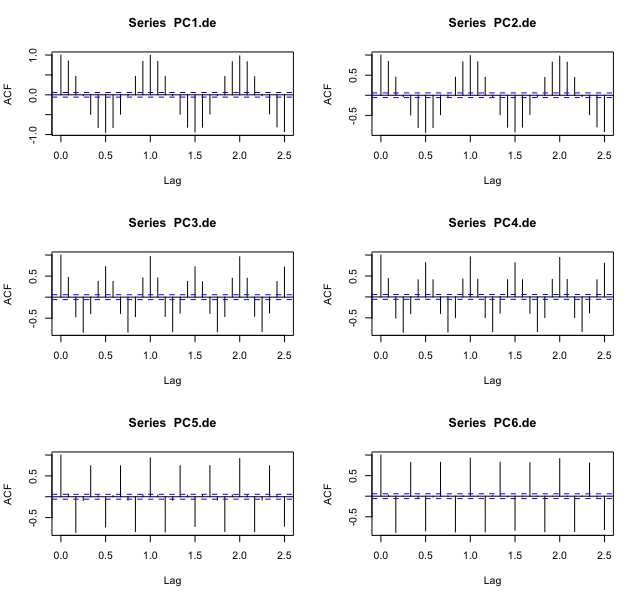
\includegraphics[width=0.7\linewidth]{../img/PCAde_ACF}
	\caption{Auto-Covariance Function}
	\label{fig:pcadeacf}
\end{figure}

\begin{figure}
	\centering
	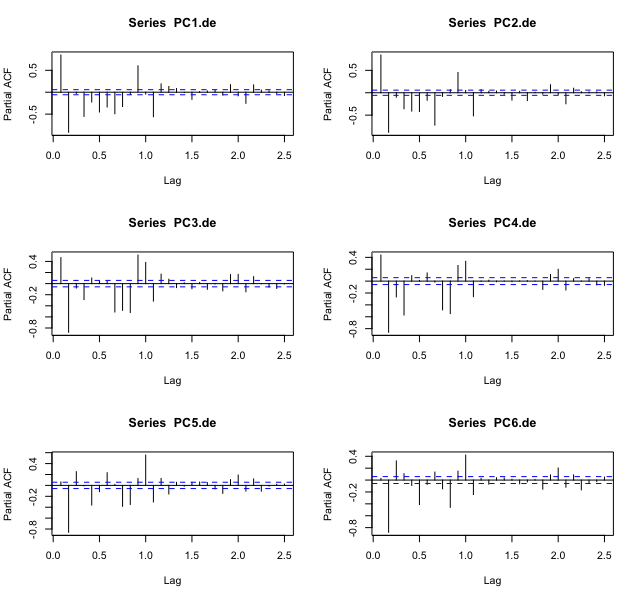
\includegraphics[width=0.7\linewidth]{../img/PCAde_pacf}
	\caption{Partial ACF}
	\label{fig:pcadpeacf}
\end{figure}

\begin{figure}
	\centering
	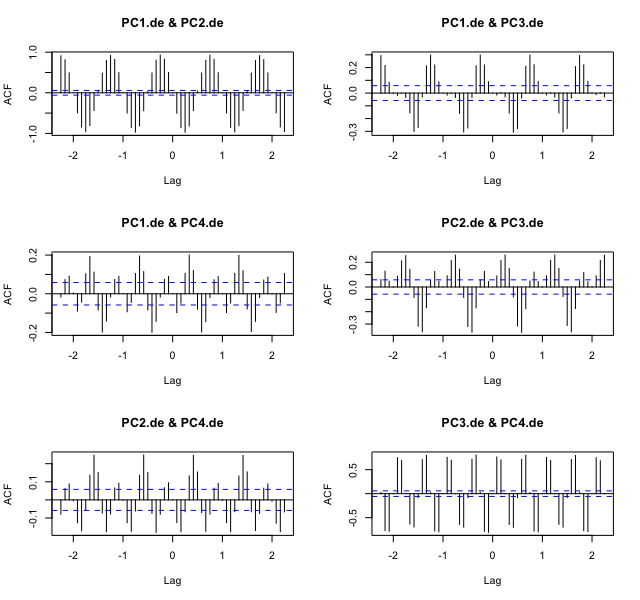
\includegraphics[width=0.7\linewidth]{../img/PCAde_CCF}
	\caption{Cross-Covariance Function}
	\label{fig:pcadpeccf}
\end{figure}

\begin{figure}
	\centering
	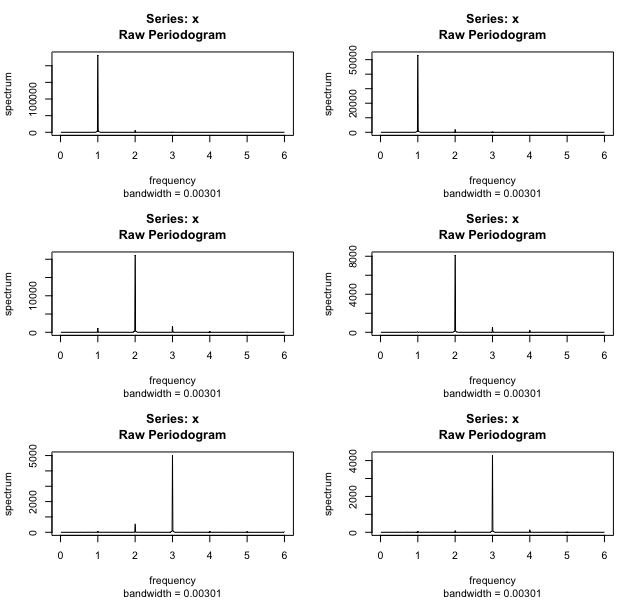
\includegraphics[width=0.7\linewidth]{../img/PCA_periodogram}
	\caption{PCA Periodogram}
	\label{fig:pcaperiodogram}
\end{figure}

\begin{figure}
	\centering
	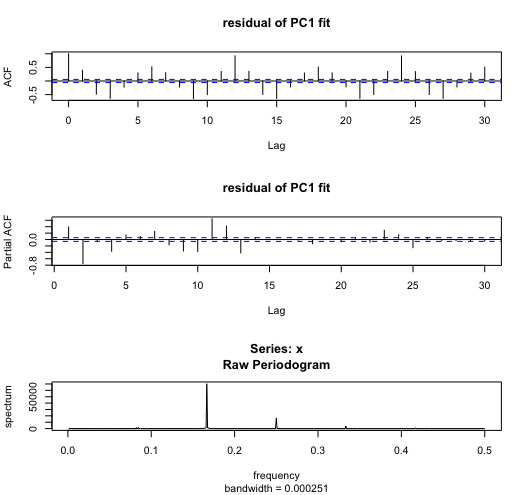
\includegraphics[width=0.7\linewidth]{../img/residualpc1}
	\caption{Analysis on Residuals PC1 Fit}
	\label{fig:residualpc1}
\end{figure}

\end{document}
